\documentclass[
class = book,
zihao = -4,
font = noto,
paper = a4paper,
openany
]{easybook}

\usepackage{xju}
\newcommand{\ti}{Ti6Al4V}

\begin{document}
	\hypersetup{pdftitle=热处理温度及冷却速度对Ti6Al4V组织和力学性能的影响,pdfauthor=田欣洋,pdfsubject={材料科学,金属学,钛合金},pdfkeywords={热处理,固溶,时效,组织},pdfstartview=FitB}
	\maketitle
	\frontmatter*[roman]

	\begin{abstract}
	\ti 合金又名TC4合金,拥有较好的塑韧性、耐热性、成形性、耐蚀性等,
%	其使用量已占钛合金使用总量的75$ \% $~85$ \% $,也是大多数高强钛合金的基础,被誉为钛合金中的“王牌合金”,
	在机械、军事、航空航天等领域获得了极为广泛的应用。但TC4合金仍存在硬度较低、摩擦磨损系数高、耐磨性能差、较低的塑韧性和力学性能上的各向异性等缺点,制约了其进一步的应用。结构决定组织,组织决定性能。合金的显微组织显然不能轻易被各种冷塑性变形所改变,而热处理恰恰具有这种控制结构、组织的能力。热处理制度的不同会带来不同的组织,进而得到各异的性能。对Ti6Al4V合金而言,普通处理方式得到的合金存在着硬度低、摩擦性能差的缺点,经过调研\ti 合金近几十年的研究可以发现固溶+时效处理是一种不错的强化手段,可以很好地调控合金的显微组织,提高强度、硬度与耐磨性,从而大幅改善构件的性能。

	本文通过固溶时效处理Ti6Al4V合金的强度性能研究,分析了不同固溶时效工艺参数下处理Ti6Al4V合金的力学性能,旨在确定最佳的固溶温度、时效温度、失效时间等参数,为工程应用提供参考。 本文全面系统地描述了950 ℃附近固溶处理、550℃附近时效处理所得的Ti6Al4V合金在室温下$ 10~240 N $施加载荷范围内的力学性能与组织特征。在不同的参数下,确定合金的强度、硬度等力学参数,分析高性能的\ti 合金所处的工艺参数范围。并结合金相特征和电子显微镜分析测试结果,通过分析合金微观组织特征和力学性能变化,探索固溶体组织转变的机理。主要研究成果如下\footnote{{\color{red}\faBan} 以下几点为胡诌,待实验结束后再整理之!}:
	\begin{enumerate}
		\item (\text{\color{blue}从热处理制度})在950℃进行固溶、550℃进行时效处理时可以得到合金最佳的力学性能。
		\item (\text{\color{blue}从微观组织})冷却速率越高,得到组织所含$ \beta  $相含量越多,综合性能越好。
		\item (\text{\color{blue}从转变机理})时效时间越久,亚稳定$ \beta $相分解的就越充分,得到的组织性能更好。
	\end{enumerate}
	\keywords{热处理,固溶,时效,组织,钛合金,工艺}
	\end{abstract}

	\tableofcontents
	\mainmatter*

	\pagestyle{Xju}
	\chapter{绪论}
\section{钛工业的发展历程与国内外现状}

钛(Titanium),原子序数为22,最早于1791年由格雷戈尔在英国康沃尔郡发现,是一种银白色的金属,具有密度小、比强度高、耐高温、化学性质性质稳定等明显优于传统金属的特性而备受重视。钛及钛合金常用来制造飞机、火箭等航天机械,一直以来都是航空航天工业的“脊柱”之一,被誉为“太空机械”\cite{XJYS200102014}。与纯钛一同发展起来的钛合金也毫不逊色,钛合金是在纯钛的基础上添加了各种各样的合金元素而形成的合金,凭借其更高的强度、耐蚀性、抗高温性能,得到了广泛的应用,尤其是在机械制造、航空航天、化工、军工等领域,钛合金的占比更大。钛工业的发展水平在一定程度上是衡量一个国家航空航天、汽车工业等领域发展水平的重要标志\cite{HSJJ202109005}。

\subsection{钛与钛合金的特点}
钛合金具有密度小,强度高的显著特点,相较于高强度钢而言,不仅强度相差无几,而且还具有更大的比强度。

\begin{table}[htbp]
	\centering
	\label{sec:bqd}
	\caption{不同合金比强度比较表}
	\begin{tabular}{ccccc}
		\toprule
		\textbf{合金} & \textbf{镁合金} & \textbf{铝合金} & \textbf{高强钢} & \textbf{钛合金} \\
		\midrule
		比强度 & 16 & 21 & 23 & 29 \\
		\bottomrule
	\end{tabular}
\end{table}

钛合金的特点如下\cite{1997titanium}:
\begin{enumerate}
	\item 熔点高。钛的熔点为1660℃,比铁的熔点还高出120℃左右。此外,在钛中加入铝、锆、锡等合金元素后,可以提高其热强性。
	\item 弹性模量低,屈服强度高,适合做弹簧材料。高端赛车内部的弹簧大多数都是由钛合金制成。
	\item 具有良好耐磨性、耐腐蚀性。钛表面易生成致密的氧化层,在氧化性或中性介质中有较强的耐腐蚀能力。
	\item 化学活性高。当钛加热到500℃以上时,氧化膜变得稀松且易脱落,在熔融状态下,极易发生自然。
	\item 特殊性能多。某些类型的钛合金还具有储氢、超导、低阻尼性,生物相容性、形状记忆 、 超弹 、高阻尼等特殊功能。
\end{enumerate}

\subsection{国外发展}
钛工业的发展充满曲折。从钛元素的发现(1791)到第一次制得较纯的金属钛(1910)经历了120年的历程。又由实验室第一次获得纯钛(1940)到首次进行工业生产,又花费了近30年的时间。
钛在自然界中主要以钛矿石的形式存在,如钛铁矿、金红石(TiO2)等,需要进行精炼(refining)才能获得纯金属。起初,钛的提取是通过高温还原法,但这种方法费时费力,成本高昂。直到了二十世纪四十年代,一种利用氯化钛矿与氯气进行反应来制备四氯化钛,然后通过还原反应(比如Na、Mg等)来得到纯钛的精炼工艺方法终于以其低廉的成本、高效的回收率得到了广泛的商业化应用。

第二次世界大战之后,世界上许多国家都开始意识到钛工业的重要性,钛工业在数年间便迅速发展成为航空、航天、军事等领域的关键材料。1954年,美国成功研发出Ti-6Al-4V合金,该合金在耐热性、强度、塑性、韧性、耐蚀性和生物相容性等方面均达到较高水平,凭借性能上的优势,\ti 迅速成为钛工业的主要合金,现已占据全部用钛量的50%以上,甚至可以说,许多其他型号钛合金不过是Ti-6Al-4V的改良版而已\cite{COLO200102000}。

\subsection{国内发展}
我国的钛工业发展起源于20世纪50年代,在六七十年代,我国成为了全球第四个建立完整钛工业体系的国家。自21世纪以来我国钛工业进入高速发展阶段,产能与产量已经连续多年占据世界第一的位置,目前海绵钛产量占全球比重已经达到六成,钛加工材产量稳定增长,钛产品消费端需求旺盛\cite{JSTB202209001},无论是在生产还是在加工领域均保持在世界前列。2014年,浙江余杭高端钛材的研发投产,标志着中国彻底摆脱了对国外的依赖,填补了中国高端钛材的技术空白。\cite{TGYJ200405004}

目前,我国的钛产品消费正处于上升期,如工业、航空航天、海洋船舶和体育休闲等中高端领域的钛材料的需求量平均增长约20%,而医疗行业受疫情影响,需求有所减少,电力和制盐等行业仍有小幅增长,整体盈利水平也有所改善\cite{BJKY202204004}。
%--------------------
%-------------------
%------------------
%------------------
%------------------

此外,近年来计算机技术的发展也为钛工业带来了新的发展机遇。计算机模拟技术用于优化钛合金的生产工艺,显著提高了产品质量。邵一涛等人利用BP人工神经网络的方法,构建了TC17钛合金组织和性能之间的关系模型,解决了传统BP人工神经网络的过拟合问题,从而获得更高的预测精度\cite{BP};李淼泉等人对 TC6 合金叶片在等温锻造过程中初生$\alpha$晶粒尺寸的演变进行了数值模拟\cite{Moni},将有限元法与 Yada 微观组织模型结合起来,并给出了 TC6 合金叶片在等温锻造过程中初生$\alpha$相的分布和晶粒尺寸的变化。在未来,随着物联网、大数据、人工智能、AIGC等技术的不断发展,钛工业也将迎来更多新的机遇和挑战。
\subsection{应用领域}

\begin{itemize}
\item  在航空航天领域,大型客机的设计制造推进迅速,同时军用飞机也在不断更新换代,因此全球钛合金的需求量也在急速增长。
\item  在医疗健康领域,钛合金材料有着良好的生物相容性,可以降低人体对植入物的排斥反应和感染风险,因此广泛用于人工关节、牙科种植体和其他医疗设备的制造。
\item  在汽车制造领域,高级车型的制造中广泛采用了钛合金零部件,以降低整车自重,提高燃油效率和汽车的运行性能。此外,钛合金耐腐蚀性好也能延长汽车零部件的使用寿命。
\item  在建筑工程领域,钛合金广泛应用于大型建筑的外墙幕墙、顶棚和立面系统中。这种材料具有优秀的耐候和抗腐蚀性能,可抵御各种恶劣气候的侵蚀,并且具有高度的可塑性和装饰性,可以为建筑带来更加优美的外观效果。

\end{itemize}
\section{钛合金的分类}
\label{sec:1.1}
因为纯钛的强度较低,限制了其在工业生产中的应用范围。钛合金是通过在纯钛中添加一些合金元素来提高其强度、耐腐蚀性等性能而形成的。常用的合金元素有铝、钒、锆、锂、铁、铜、镍等,通过调整元素配比和控制制备工艺,可以获得适合不同领域应用的各种高性能钛合金材料。

\subsection*{合金元素}
工业钛合金的主要合金元素为铝、钒、钼三种,此外还有Cr、Mn、Fe、Cu、Sn、Zr、W等元素组成,可以根据合金元素对钛多晶型转变温度的影响可将其分为三大类:$\alpha$稳定元素、$\beta$ 稳定元素、中性元素,形成的四种类型的相图示意图如图1.1所示。
\begin{figure}[h!]
	\centering
	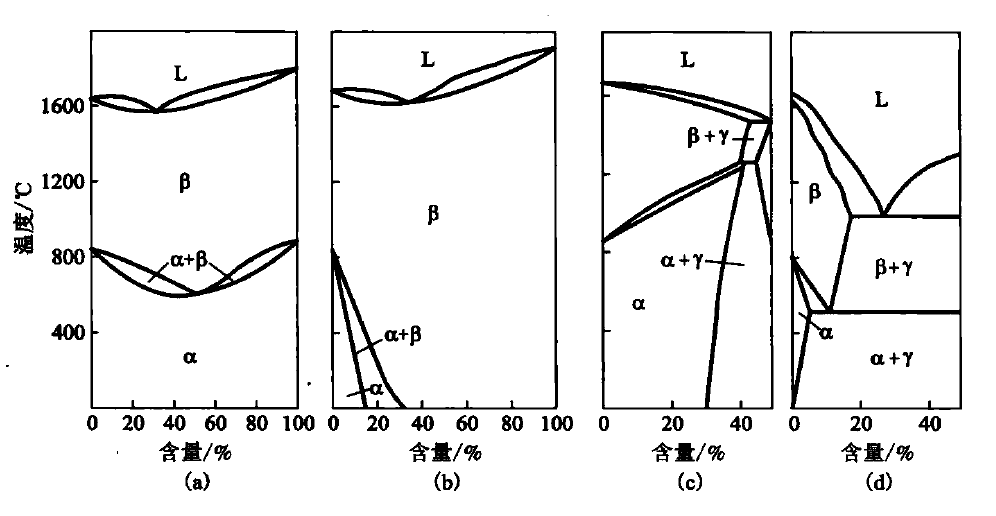
\includegraphics[width=0.9\linewidth]{pic/01}
	\caption{合金元素对钛合金相图的影响示意图}
	\label{fig:01}
\end{figure}

工业上一般根据$\beta$相稳定元素系数$K_{\beta}$来划分不同的合金元素,$K_{\beta}$是指合金中各$\beta$稳定元素与各自的临界浓度的比制之和,即:
$$
K_{\beta}=\frac{ C_{1} }{C_{k1}}+\frac{ C_{2} }{C_{k2}}+\frac{ C_{3} }{C_{k3}}+\cdots+\frac{ C_{n} }{C_{kn}}
$$
根据 $\beta$ 相稳定系数划分合金类型为:
\begin{enumerate}
	\item  $\alpha$ 型合金 $K_\beta$ 为 $0 \sim 0.07$
	\item 近 $\alpha$ 型合金 $K_\beta$ 为 $0.07 \sim 0.25$
	\item $\alpha+\beta$ 型合金 $K_\beta$ 为 $0.25 \sim 1.0$
	\item 近 $\beta$ 型合金 $K_\beta$ 为 $1.0 \sim 2.8$
	\item $\beta$ 型 合金 $K_\beta$ 为 > 2.8
\end{enumerate}
\subsection*{(1)$\alpha$型}
经退火处理后,$\alpha$型钛合金的组织通常存在单相的$\alpha$固溶体,或者以含微量金属化合物的$\alpha$固溶体的形式存在。其主要合金元素包括铝、锡、锆等$\alpha$稳定元素,以及钒、钼、铌等中性元素,各个元素都可以起到固溶强化的作用,因此这些元素都被广泛地应用于钛合金的制备中。

常用的$\alpha$型钛合金包括TA2(工业纯钛)、TA9(Ti-0.2Pb)、TA10(Ti-0.3Mo-0.8Ni)等。

$\alpha$型钛合金的$\beta$相转变温度较高,因而具有良好的热强性、高温稳定性。焊接性性能好,并在高温环境下具有极好的组织稳定性和抗蠕变性能,在低温环境下也依然保持良好的延展性,因而适合制作各种飞行器形状复杂的外层板材。但它对热处理和组织类型不敏感,故不能采用热处理的方式强化其组织\cite{TiandAl}。
\subsection*{(2)$\beta$型}
$\beta$型钛合金主要包含钒、钼、铌、钽等$\beta$相稳定元素,若在合金中加入少量的铝、锆、锡等元素,则可以提高$\beta$型钛合金的塑性,并且改善其热稳定性。这些合金元素的加入可以控制合金的相转变温度,使其具有更加优异的力学性能和高温耐久性。
常见的$\beta$型钛合金有TB2(Ti-5Mo-5V-8Cr-3Al)、TB6(Ti-10V-2Fe-3Al)、TB7(Ti-36Mo)等。

与$\alpha$型、$\alpha+\beta$型钛合金相比,$\beta$型钛合金的显微组织通常更粗大。该合金具有良好的冷成形、冷加工性能,较好的淬火态塑性以及可焊接性。但是,亚稳态$\beta$型钛合金的热稳定性较差。$\beta$型钛合金中含有较高的$\beta$稳定元素,主要分为稳定$\beta$型钛合金和亚稳定$\beta$型钛合金。稳定$\beta$型钛合金在平衡状态下全部由稳定的$\beta$相组成,经热处理后不易产生变化。
\subsection*{(3)$\alpha$+$\beta$型}
经过退火处理的$\alpha+\beta$型钛合金在室温下具有不同比例的$\alpha$和$\beta$相组织,其锻造和轧制等加工成型性能比$\alpha$型、$\beta$型钛合金更加优异。合金中除了含有定量的铝元素外,还含有少量的其他元素,可以通过适当的热处理方法对$\alpha+\beta$型钛合金进行组织强化。其强度和淬透性随着$\beta$相稳定元素含量的增加而提高。

最常用的$\alpha$+$\beta$型钛合金包括TC4、TC6、TC12等,其中TC4钛合金(等轴马氏体型两相合金)作为做早被应用的钛合金,该合金以其优越的性能占据了钛工业的大量市场,现在占到 Ti 合金总产量的 50$ \%  $, 占到全部Ti 合金加工件的95$ \% $ 。

从成分上来看,这类钛合金中的合金元素基本上是以铝为主要合金元素,$\beta$稳定化元素为辅助元素。这使得$\alpha$+$\beta$型钛合金组织变动的余地较为灵活,性能变动范围大,可以满足各种应用场合及工况要求\cite{TiandAl}。
\section{钛合金的显微组织}
众所周知,材料的最终性能是由显微组织的形态决定的, 不同的组织对应于不同的力学性能, 而微观组织形态主要取决于合金的化学成分、变形工艺和热处理方式等。

如前所述,钛合金的基本组织由密排六方的低温$\alpha$相和体心立方的高温$\beta$相构成。除少数稳定$\beta$型钛合金外,体心立方的高温$\beta$相一般难以保留到室温,会在冷却过程中发生$\beta$相向$\alpha$相的多晶转变,并以片状形态从原始$\beta$晶界析出。片状组织主要由片状$\alpha$和片状$\beta$相构成,与母相之间存在着一定的结晶学位向关系,称为$\beta$转变组织。在$\alpha+\beta$两相区受到足够大的塑性变形后,片状组织可再结晶球化得到等轴组织。因此,根据晶内$\alpha$相的形状变化,$\alpha+\beta$型钛合金的显微组织大致分为四类:

\begin{itemize}
	\item 	\textbf{等轴组织}:在$\beta$转变温度以下30~100摄氏度加热,在充分的塑性变形和再结晶退火后可以形成等轴组织。具有良好的塑性、延伸率和较高的断面收缩率,同时热稳定性也很高,综合性能优良。
	\item 	\textbf{网篮组织}:在 $\beta$ 区加热或开始变形, 在 $\alpha+\beta$ 两相区的变形量不太大时形成。具有高的持久强度和蠕变强度,在热强性方面具有明显的优势,具有高的断裂韧性、低的疲劳裂纹扩展速率。缺点是塑性和热稳定性较低。
	\item 	\textbf{双态组织}:在 $\alpha+\beta$ 两相区的上部加热或者进行变形可以获得。双态组织兼顾了等轴组织和片状组织的优点, 等轴 $\alpha$ 含量在 $20 \%$ 左右的双态组织具有强度 - 塑性 - 韧性 - 热强性的最佳综合匹配。与片状组织相比, 双态组织具有更高的屈服强度、塑性、热稳定 性和疲劳强度; 与等轴组织相比, 双态组织具有较高的持久强度、蜻变强度和断 裂韧性, 以及较低的疲劳裂纹扩展速率 $\mathrm{d} a / \mathrm{d} N$ 。
	\item 	\textbf{魏氏组织}:在较高温度的 $\beta$ 区加热或变形量不够,时可以形成。魏氏组织具有最高的蠕变抗力、持久强度和断裂韧性, 但是其致命的弱点是塑性低, 尤其是断面收缩率远低于其他组织类型。类似于钢中的过热组织, 在实际生产过程中没有特殊的需求应尽量避免。
\end{itemize}

\begin{table}[htbp]
	\centering
	\label{sec:detial}
	\caption{不同组织的性能}
	\begin{tabular}{ccccc}
		\toprule
		机械性能 & 抗拉强度 $ \sigma$ MPa & 延伸率 $\delta\%$ & 冲击韧性& 断裂韧性 \\  \midrule
		片层组织 & 1020 & 9.5 & 355.3 & 102 \\
		网篮组织 & 1010 & 13. 5 & 533 & - \\
		双态组织 & 980 & 13 & 434.3 & - \\
		等轴组织 & 961 & 16.5 & 473.8 & 58.9 \\ \bottomrule
	\end{tabular}
\end{table}
\section{钛合金的相变}
钛合金中的相变主要包括:多晶转变、共析转变、有序化、亚稳相等稳转变、非等温转变等。

%	众多研究者已将钛合金的相变类型绘制成了一个表格:
%	\begin{table}[htbp]
	%	\centering
	%	\label{sec:change}
	%	\caption{相变过程}
	%		\begin{tabular}{ccc}
		%			\hline
		%			编号 & 相变 & 过程 \\ \hline
		%			I & 淬火过程中$\beta$相的分解 & (1)钛的马氏体:$ \beta $ 	o $\alpha^{'}$ , $\alpha^{"}$\$ \\ \hline
		%	~ & 淬火过程中$\beta$相的分解 & (2)无热\$$\backslash$omega\$相:\$$\backslash$beta $\backslash$to $\backslash$omega\_\{$\backslash$text\{无热}} +$\backslash$beta\$ \\ \hline
%II & 等温转变中$\beta$相的分解 & (1) \$$\backslash$beta($\backslash$beta+$\backslash$alpha)$\backslash$to a\^\{"},a\^\{"}$\backslash$text\{富},a\^\{"}$\backslash$text\{贫}\$ \\ \hline`
%~ & 等温转变中$\beta$相的分解 & (2) \$$\backslash$beta\^\{'}$\backslash$beta$\backslash$text\{富},$\backslash$beta$\backslash$text\{贫}\$ \\ \hline
%III & 残余$\beta$相分解 & (1)      相离析: \$$\backslash$beta\_\{$\backslash$text\{残}} $\backslash$to $\backslash$beta\^\{'}+$\backslash$beta\$ \\ \hline
%\end{tabular}
%\end{table}

由于$\beta$钛合金的用途更为广泛,本设计侧重于对$\beta$合金进行说明。众所周知,$\beta$钛合金按照亚稳定状态相组成可分为3类 :稳定$\beta$型钛合金 、 亚稳定$\beta$型钛合金和近$\beta$型钛合金。其中亚稳态$\beta$合金的综合性能最好,其相变过程也最复杂。


\subsection*{亚稳定$\beta$相的分解}
亚稳定$\beta$相的分解的分解过程如下:
\begin{enumerate}
	\item  当加热温度较低时,$\beta$相将分解为无数极小的溶质原子贫化区$ \beta^{'} $和与其相邻的溶质原子富集区$\beta$。
	\item  随着加热温度升高或加热时间延长,则根据$\beta$相化学成分不同而从溶质原子贫化区中析出w相或$ \alpha^{"} $相。
	\item  最后在贫化区析出的$ \alpha^{"} $和w相分解为平衡的$\alpha$和$\beta$相。
\end{enumerate}

出现这种逐步分解的原因就在于虽然成分范围宽广的钛合金,通过快速冷却$\beta$相可以保持在亚稳定状态,随后在高于室温的温度下逐渐分解,但是在温度不太高的情况下,由于密排六方点阵的$\alpha$相在体心立方点阵的$\beta$相基体中生核比较困难,而一些中间分解产物比较容易生核,因此,亚稳定$\beta$相不能直接分解形成平衡的$\alpha$相,而是经过一些中间分解过程,由生成的一些中间分解产物(或称过渡相)再转变为平衡的$\alpha$相。至于形成哪一种过渡相,取决于加热温度和合金成分。
% 内容删减第一弹
%最常见的过渡相是等温相和$\beta$’相。在500℃范围内加热时,亚稳定$\beta$相的分解过程为:
%\begin{enumerate}
%	\item  $\beta$亚稳→$\beta$'+$\beta$→a"+$\beta$→a+$\beta$
%	\item  $\beta$亚稳→$\beta$'+$\beta$→ω+$\beta$→a+$\beta$
%\end{enumerate}
%
%\subsection{马氏体相变}
% 钛合金自高温快速冷却时, 视合金成分不同, $\beta$ 相可转变为马氏体 ( $\alpha^{\prime}$ 或 $\left.\alpha^{\prime \prime}\right) 、 \omega$ 相或过冷 $\beta$ 相。在快速冷却过程中, 由于从 $\beta$ 相转变为 $\alpha$ 相的过程来不及进行, $\beta$ 相将转变为成分与母相相同、晶体结构不同的过饱和固溶体, 即马氏体。
%
%
% 我们知道马氏体转变是一种切变相变。在钛合金中发生马氏体转变时, $\beta$ 相中的原子作集体的有规律的近程迁移, 迁移距离较大时, 形成六方 $\alpha^{\prime}$ 相; 迁移距离较少时, 形成斜方 $\alpha^{\prime \prime}$ 。当 $\beta$ 相中的合金元素含量较少时, 原子位移较大, 点阵改组进行到底, 得到密排六方 $\boldsymbol{\alpha}^{\prime}$ 相; 当合金元素含量较大时, 点阵改组受到阻碍, 停留在某一中间阶段, 即形成斜方点阵 ( $\alpha^{\prime \prime}$ 相)。
%
%\subsection{ ω相变}
%合金成分在临界浓度$C_0$ 附近的合金从高温淬火后 , 将在合金组织中形成一种ω相。ω相可以根据组织分为两类——无热ω相与等温ω相。
%
%\begin{enumerate}
%	\item 无热ω相:当$\beta$合金元素的成分范围达到某一临界值时,合金在$\beta$相区淬火可以得到ω相。其特点是尺寸小,硬度大,脆性极大,会使材料的塑韧性急剧降低,当其含量达到80$ \% $时,合金就会失去宏观塑形。可以通过改变化学成分或者回火工艺予以控制。
%	\item 等温ω相:在淬火得到的亚稳定$\beta$相后,在随后的时效过程中,会出现$\omega \to \beta$转变,时效温度一般在100~500℃之间,相对于无热ω,$\beta$相分解为等温ω相的速度最快。其尺寸较小晶粒密度大,有方形和椭球形状两种形态,其含量越多,合金的硬度越高,塑韧性越差,当含量大约为50$ \% $时合金的综合性能较好。
%\end{enumerate}
%
%\subsection{$\alpha$相的形成}
% 在相分离和ω相变不能出现的高温时效过程中,亚稳$\beta$相可以直接转变为$\alpha$相,进而转变为$ 1\alpha $和$ 2\alpha $两种相
%
%%\begin{enumerate}
%%	\item  在位错及亚晶界上直接形成$\alpha$相;
%%	\item  经过过渡相形成a相
%%	\item  $\beta$→$\beta$'(bcc,贫溶质)→1$\alpha$和2$\alpha$;
%%	\item  $\beta$→ω(hcp,贫溶质)→l$\alpha$和2$\alpha$。
%%\end{enumerate}
%其中,1$\alpha$相为片层状,2$\alpha$为透镜状,但两者的晶体结构并无区别。
%在$\beta$相的时效转变中,有可能生成$\beta$'、ω、1$\alpha$和2$\alpha$相沉淀。$\beta$相对合金的强度无明显改善,相虽能强化合金,但会强烈降低合金的韧性。因此工业上的$\beta$合金都设计成使$\alpha$相(1$\alpha$和2$\alpha$)作为基体中的硬化沉淀相,合金的强度则由时效形成的$\alpha$相粒子尺寸、形状及体积分数控制。有实验数据表明,当合金中出现非共格的、有较大体积分数的、尺寸较大的2$\alpha$型沉淀时,合金将有良好的综合性能。


%\section{钛合金组织分析方法}

\section{\ti 合金研究进展}
近些年来国内对于\ti 合金的研究,主要在热处理工艺上取得了较多成果\cite{guokaiTC4taihejinrechuligongyideyanjiuxianzhuangjijinzhan2021}。

\begin{enumerate}
	\item 固溶处理:实施固溶处理工艺,是为了得到等轴稳定的$\alpha$相、马氏体弥散的$ \alpha^{'} $相、亚稳定状态的$\beta$相,等轴的$\alpha$相能够让合金的力学性能得到综合性的提升,马氏体弥散的$ \alpha^{'} $相能够让合金,在强度、硬度上得到提高,塑性、韧性被降低\cite{gurong2002}。
	\item 时效处理:有研究\cite{luyuanyuanShixiaochuliduiTC4taihejinweiguanzuzhihelixuexingnengdeyingxiang2019}发现,次生的$\alpha$相体积分数在TC4钛合金中,会对屈服强度产生很大的影响。在条件相等的情况之下,时效温度越低组织越小,时效温度高低组织越大。研究人员主要是通过控制参数,来影响对次生$\alpha$相的含量,从而来实现TC4钛合金在力学的性能上得到更好的提升。
	\item 深冷处理:深冷处理是近些年来新兴的一种处理工艺,其可以对金属内部的组织进行改善,在进行深冷处理的时候操作比较方便,对环境也不会造成太大的污染,并且能够让在热处理之后残留的奥氏体被清除掉。实验研究发现,原始的$\beta$相会在深冷处理的过程当中,逐渐的向$\alpha^{'}$相去转变,残余应力在组织中会变少,与此同时网篮状组织的增加,会让TC4钛合金的韧性、强度、塑性,在组织上的性能得到提高。
\end{enumerate}

\section{研究背景意义与研究内容}
\subsection{研究意义}
\ti 合金具有比强度高、生物相容性好、耐高温、化学性质性质稳定,等优良特性,在航空航天、汽车工业、医疗健康领域等领域得到了广泛应用,是目前应用最广泛的钛合金。但其室温塑性较低,加工硬化能力较差,冷加工成型困难。目前相关研究中,提升TC4钛合金室温塑性的手段主要包括\textbf{添加合金元素}、\textbf{剧烈塑性变形}和\textbf{相变热处理}。虽然前两种处理工艺对于合金的塑性提升明显,但工艺复杂、成本较高\cite{miao},而第三种热处理方法则工艺简单,成本较低,是提升TC4合金性能的不二之选。

钛合金的热处理方式属于共析和有序化转变,在退火和时效过程中存在共析 转变,时效过程中存在有序化转变,现阶段\ti 合金的基本热处理工艺主要有:深冷处理、固溶处理、渗氮处理等。不同的热处理工艺互相组合可以对合金产生更好的强化效果,现阶段工业上常采用\cite{zhoukaixiangJiyushenlengchulidenanjiagongcailiaoqiexiaotexingyanjiu2022}:淬火+时效;固溶+时效;双重固溶+时效;固溶+双重时效;时效+冷轧+低温氮化等,其中固溶+时效处理是应用最为广泛的一种热处理工艺组合。但是目前对于固溶+时效处理方法的最佳工艺参数一直没有定论,本设计的目的就是确定\ti 合金最佳的固溶+时效热处理工艺参数,并分析参数对于合金组织与力学性能的影响。

\subsection{研究内容}
本设计通过对TC4钛合金进行多种不同工艺参数的热处理,来重点研究不同固溶温度和冷却方式、时效的温度和时间下,TC4合金显微组织与力学性能的变化规律,重点关注$ \beta  $相稳定性变化及其对钛合金加工硬化和塑性的影响,以期为实际生产中探索高塑性TC4钛合金加工工艺提供理论依据。
设计的具体内容是:从\ti 合金板材中切取试样,采用\text{JC-MF12-30}型箱式电阻炉进行固溶与时效热处理;将热处理好的试样,放置在万能试验机上按{GB/T228-2002}进行室温力学性能测试,以得到合金的力学性能数值;然后对试样进行打磨抛光,在光学金相显微镜下进行组织的观察;最后分析工艺参数、力学性能与微观组织的关系,得到最佳热处理的工艺参数。
\subsection{研究路线方法}
本设计采用实验+分析的研究方法,热处理在\text{\color{teal}JC-MF12-30}%\footnote{该箱式电阻炉(也称为马弗炉)制造商为$\text{青岛聚创}^\text{\textregistered}  $环保集团有限公司,设备编号为803229}
型箱式电阻炉中进行。热处理完成后,进行了断裂形态的显微组织分析、拉伸力学试验、仪器冲击试验、X射线衍射(XRD)试验和环境扫描电子显微镜(ESEM)观察,研究的路线如\ref{fig:roadmap}所示:

\begin{figure}[h!]
	\centering
	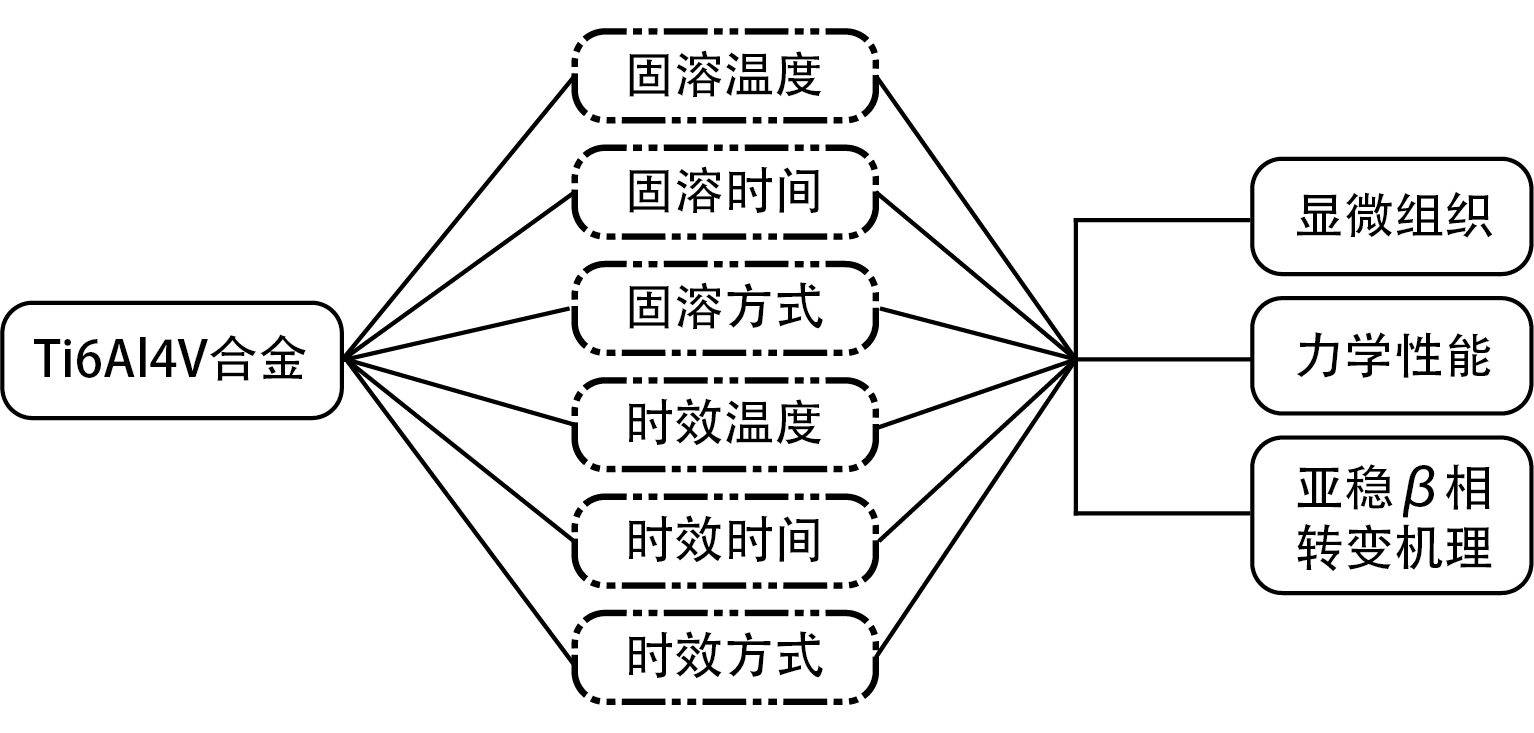
\includegraphics[width=0.8\linewidth]{pic/路线图}
	\caption{研究路线图}
	\label{fig:roadmap}
\end{figure}

	\chapter{试样材料及研究方法}
\section{材料属性与试样加工过程}
\subsection{实验材料属性}
本实验用的是真空自耗两次熔炼所得的钛合金板,其化学成分参数与室温(20℃)力学性能参数如\ref{sec:mytc4chem}与\ref{sec:mytc4machin}所示:
\begin{table}[htbp]
	\centering
	\caption{试样的化学成分参数}
	\label{sec:mytc4chem}
	\begin{tabular}{cccccccc}
		\toprule
		元素($ \% $) & Al & V &Fe &C& O& N &H \\ \midrule
		实际含量 & 6.12&4.06 &0.13 &0.012&0.112&0.009&0.004  \\
		标准要求 &$ 5.5\sim 6.75 $ & $ 3.5\sim 4.5 $&$ \le 0.30 $ & $ \le 0.05 $&$ \le 0.20 $&$ \le 0.03$ &$ \le 0.015 $ \\ \bottomrule
	\end{tabular}
\end{table}

$\beta$转变温度是钛合金的重要参数之一,它是制定钛合金的热机械工艺和热处理工艺的重要依据,相变过程如\ref{sec:Tc4betachange}所示。郭凯\cite{guokaiTC4taihejinrechuligongyideyanjiuxianzhuangjijinzhan2021}等人表示:当固溶温度高于 $\beta$ 相变时的温度时,合金的强度伴随温度的增加而下降,而且残余应力也开始大幅度的降低;当固溶温度低于 $\beta$ 相变时的温度时,合金的强度伴随温度的增加而增加,残余应力也略微提高。但是徐戊矫、谭玉全\cite{xujianGurongshixiaogongyiduiTC4taihejinzuzhijixingnengdeyingxiang2014}却表明:在相变点以下,随着退火温度的升高,材料的 强度、塑性和冲击韧性呈降低趋势。之所以会出现这种完全相反的结论,很可能是研究者对于相变点的具体值定义不清晰导致的,可见相变点的确定在固溶处理过程中是非常关键的。

近年来,确定$ \beta $相变点的常见计算方法\cite{zhuhongTaihejinaVxiangbiandiandejizhongceshifangfatantao2013}主要有:连续升温金相法、X 射线衍射法、电阻法、等热膨胀法、元素含量法和神经网络模型预测预测法\cite{renchiqiangGurongshixiaoduiTC4taihejinxianweizuzhihelixuexingnengdeyingxiang2022}等。
\begin{table}[htbp]
	\centering
	\caption{\ti 合金$ \alpha+\beta \to \beta $转变时发生的相变及存在的相}
	\label{sec:Tc4betachange}
	\begin{tabular}{ccc}
		\toprule 室温相 & 相变过程 & 高温相 \\
		\midrule$\alpha-\mathrm{Ti}$ & $\alpha-T i \rightarrow \beta-T i$ & $\beta-\mathrm{Ti}$ \\
		$\alpha-\mathrm{Ti}-\mathrm{Al}$ & $\alpha-\mathrm{Ti}-\mathrm{Al} \rightarrow \beta-\mathrm{Ti}+\beta-\mathrm{Ti}-\mathrm{Al}$ & $\beta-\mathrm{Ti}, \beta-\mathrm{Ti}-\mathrm{Al}$ \\
		$\beta- \mathrm{Ti}-\mathrm{V}$ & $\beta-\mathrm{Ti}-\mathrm{V} \rightarrow \beta^{-} \mathrm{Ti}-\mathrm{V}$ & $\beta-\mathrm{Ti}-\mathrm{V}$ \\
		\bottomrule
	\end{tabular}
\end{table}

由于能力所限,本试验采用元素含量法来进行相变点的计算:根据合金中各元素对相变温度的影响来对相变点进行推算,通过\ref{sec:chem4ti}所示\cite{ananyaLocationBasedIntelligent2011}的因素,利用经验公式\ref{jingyan}来计算。
\begin{equation}
	T_\beta=885^{\circ} \mathrm{C}+\sum \text { 各元素含量 } \times \text { 各元素含量对 }(\alpha+\beta) / \beta \text { 相变点的影响 }
	\label{jingyan}
\end{equation}
其中885℃为纯钛的相变点。
\begin{table}[htbp]
	\centering
	\caption{部分元素含量对钛合金相变点的影响}
	\label{sec:chem4ti}
	\begin{tabular}{cccc}
		\hline 元素名称 & 元素含量 $(\mathrm{Wt} \%)$ & 差值&累积值 \\
		\hline $\mathrm{Al}$ & $2.0 \sim 7.0$ & 29+$23.0^{\circ} \mathrm{C} / 1.0 \%$ & $+123.76^{\circ} \mathrm{C}$ \\
		$\mathrm{V}$ & $0 \sim 10.0$ & $-14.0^{\circ} \mathrm{C} / 1.0 \%$ & $-56.84^{\circ} \mathrm{C}$ \\
		$\mathrm{Fe}$ & $0 \sim 15.0$ & $-16.5^{\circ} \mathrm{C} / 1.0 \%$ & $-2.145^{\circ} \mathrm{C}$
		 \\
		$\mathrm{C}$ & $0 \sim 0.15$ & $+2.0^{\circ} \mathrm{C} / 0.01 \%$ &$ +2.4^{\circ} \mathrm{C} $\\
		$\mathrm{O}$ & $0 \sim 1.0$ & $+2.0^{\circ} \mathrm{C} / 0.01 \%$& $ +22.4^{\circ} \mathrm{C} $\\
		$\mathrm{~N}$ & $0 \sim 0.5$ & $+5.5^{\circ} \mathrm{C} / 0.01 \%$& $ +4.95^{\circ} \mathrm{C} $\\
		$\mathrm{H}$ & $0 \sim 0.50$ & $-5.5^{\circ} \mathrm{C} / 0.01 \%$ &$ -2.2^{\circ} \mathrm{C} $\\
		总计&&&$ +92.325^{\circ} \mathrm{C} $\\
		\hline
	\end{tabular}
\end{table}


关于$\beta$转变温度的具体值,目前广泛认同的是位于975℃附近,但是由于不同试样的合金元素的种类与含量的差异,尤其是局部化学成分的差异,使得不同研究人员实际测得的相变点温度有所差异\cite{wangtaoTC4hejinxiangbianwendujiancezhongjieguobuyizhiyuanyinfenxi2013}。

姚德人等\cite{yaoderenTc4taihejinxiangbiandiandeceding1975}表明相变温度为975℃到980℃之间,此时的合金拥有最低的硬度,当温度略大时会发生$\beta$晶粒的显著长大;相变点以下50℃以内水淬,可以得到不同数量的初生$ \alpha $和马氏体$ \alpha^{\prime} $,而后再进行低温退火时,马氏体$ \alpha^{\prime} $又会转变为稳定的次生$ \alpha$和$ \beta $,可以得到较好的综合性能\footnote{\color{red}此文章写于1975年,但是仍然非常有参考价值}。刘伟东等人\cite{liuweidongTC4hejinVzhuanbianwendudejinxiangfacedingyulilunjisuan2014}通过连续升温金相法,使用EET\footnote{Empirical Electron Theory of solids and molecules“固体与分子经验电子理论”(简称余氏理论)}模型建模测得了\ti 合金的相变温度为974.58℃;孙宇、曾卫东等人\cite{sunyuYingyongrengongshenjingwangluoyanjiuhuaxueyuansuduitaihejinxiangbiandiandeyingxiang2010}通过人工神经网络ANN技术,运用反向传播算法,建立了三层神经网路-钛合金相变预测模型,最终预测得到在绝对误差为9.8℃的情况下,TC4的相变点为994.8℃。

本设计的试样通过计算法得到的相变点温度为$ 885+92.325=977.325^{\circ} \mathrm{C} $,可见还是比较符合现实情况的。
\begin{table}[htbp]
	\centering
	\caption{试样的力学性能参数}
	\label{sec:mytc4machin}
	\begin{tabular}{cccc}
		\toprule
		力学性能& 抗拉强度$Mpa  $& 屈服强度$ Mpa $&断后伸长率$ \% $\\ \midrule
		实测值 & 983 &902 & 13\\
		标准值 &$ \ge 895 $&$ \ge 830 $&$ \ge 10 $ \\ \bottomrule
	\end{tabular}
\end{table}


为了节约成本,本设计选择了尺寸较小的试样来进行实验,整体尺寸为$ 25mm\times 7.5mm $的狗骨状片体,具体参数如\ref{fig:试样尺寸}所示:
%3-28日上午,经过老师说明,由于试样为板材,加工成圆柱较为困难,故加工成二位平面的“狗骨头”

\begin{figure}[h!]
	\centering
	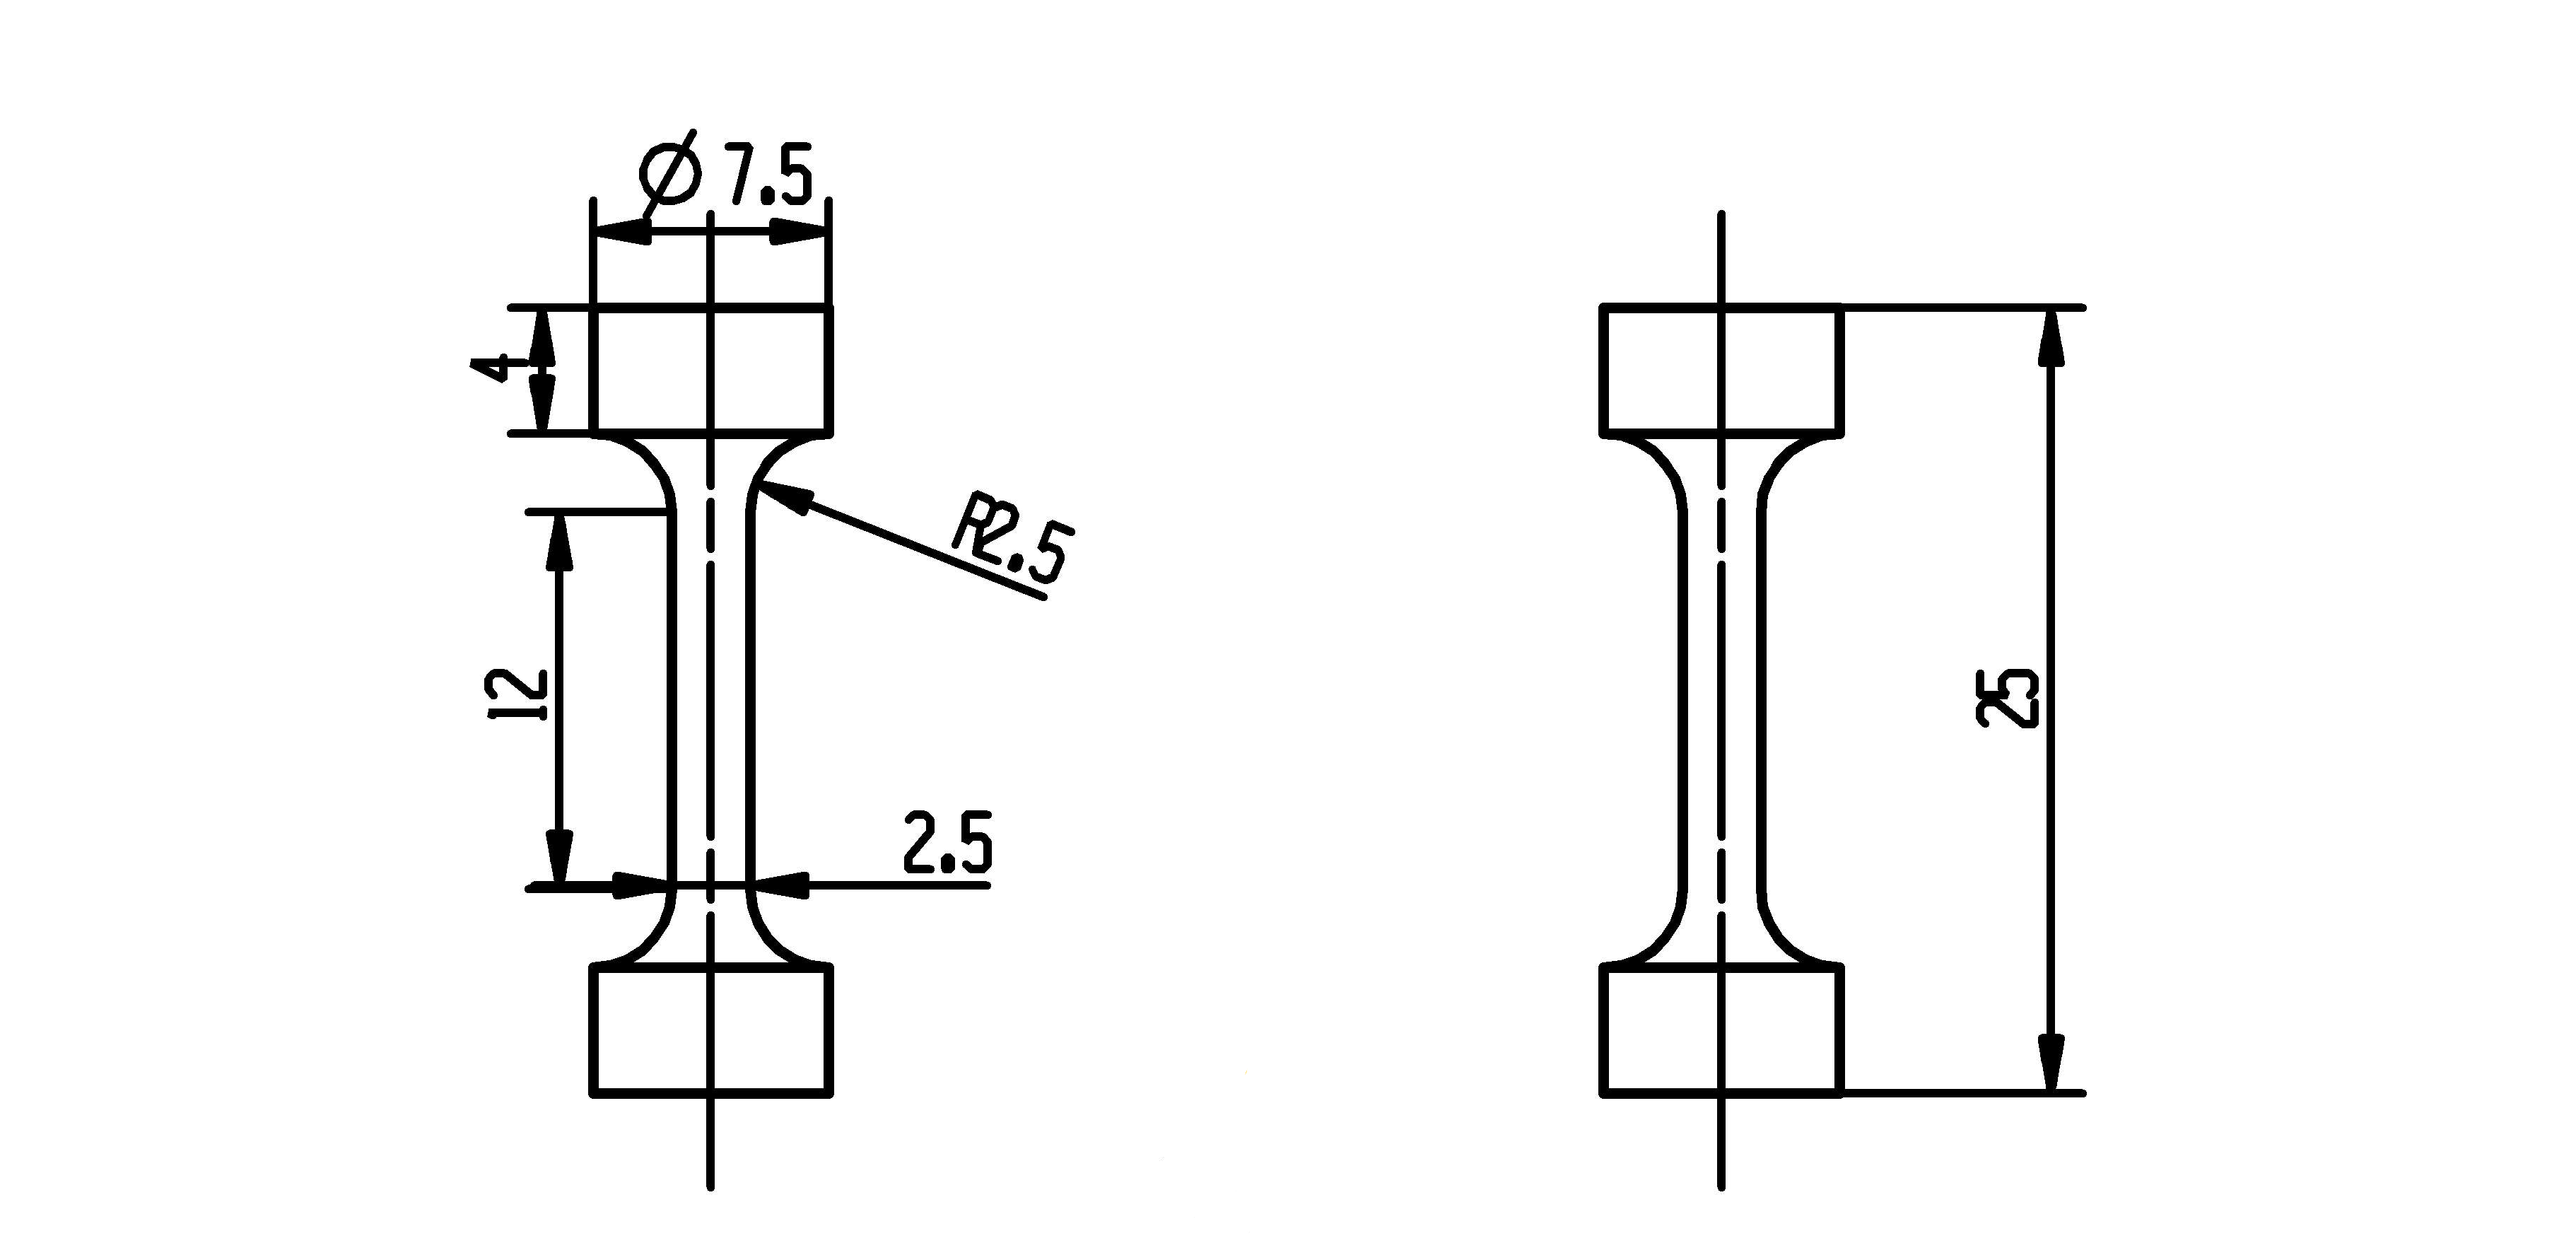
\includegraphics[width=0.99\linewidth]{pic/试样}
	\caption{试样的尺寸参数}
	\label{fig:试样尺寸}
\end{figure}

%
%\begin{figure}[!htbp]
%	\centering
%	\begin{minipage}[t]{0.68\textwidth}
	%		\centering
	%		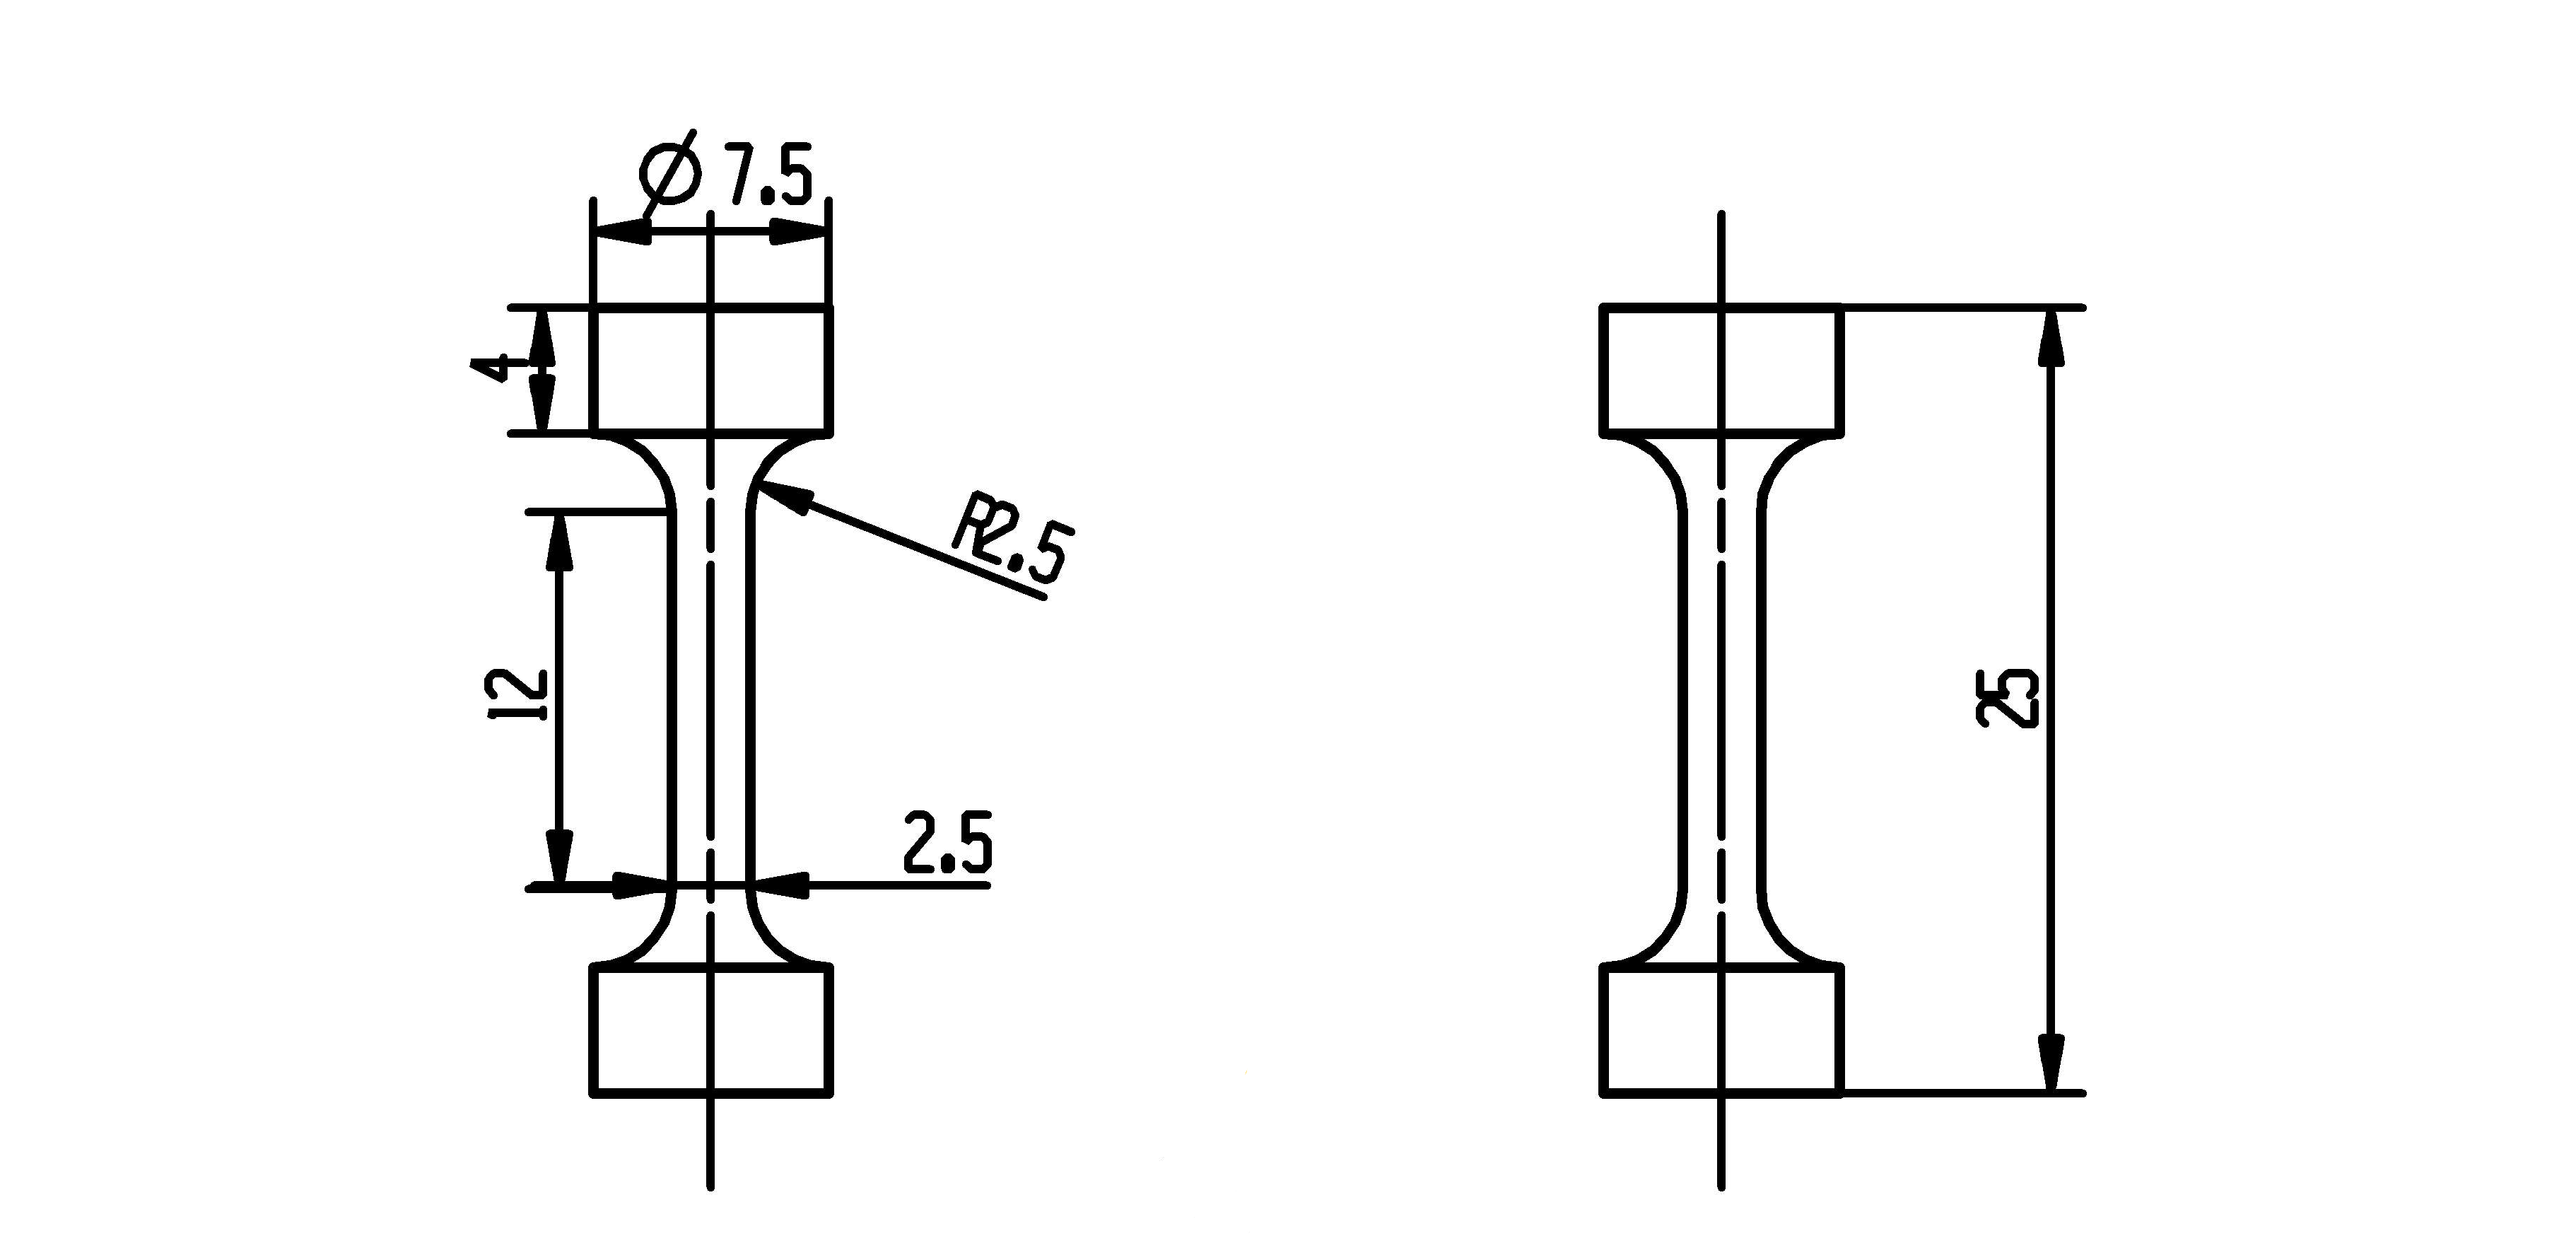
\includegraphics[width=6cm]{pic/试样}
	%		\caption{试样的尺寸参数}
	%		\label{fig:试样尺寸}
	%	\end{minipage}
%	\begin{minipage}[t]{0.3\textwidth}
	%		\centering
	%		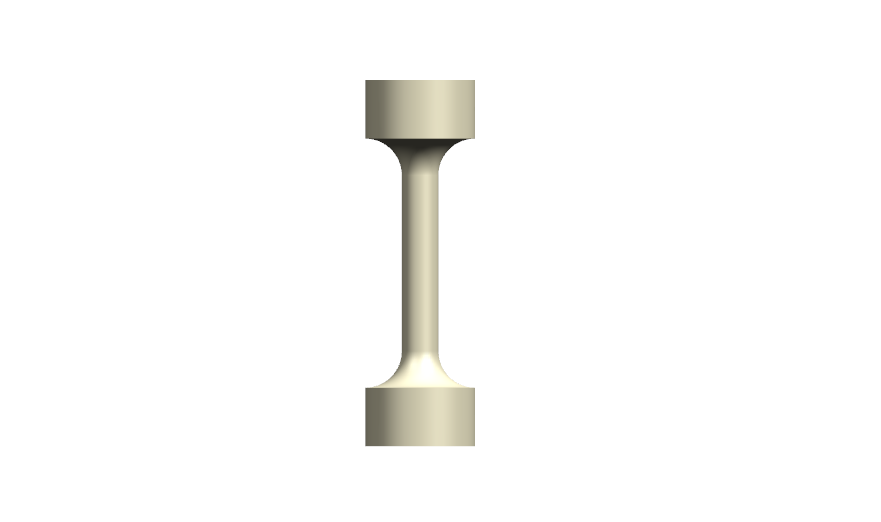
\includegraphics[width=6cm]{pic/模型}
	%		\caption{试样的三维模型}
	%		\label{fig:试样的三维模型}
	%	\end{minipage}
%%	\caption{试样参数}
%\end{figure}
\subsection{试样加工}
本设计采用电火花线切割加工(Wire cut Electrical Discharge Machining,简称WEDM)的方法进行加工。在一开始只考虑了材料的利用率,就设计了如\ref{fig:badway}所示的密集排列。但是在实际加工的时候,却发现在这样的设计方式根本不可行——没有夹具的位置,且刀路比较长。

\begin{figure}[h!]
	\centering
	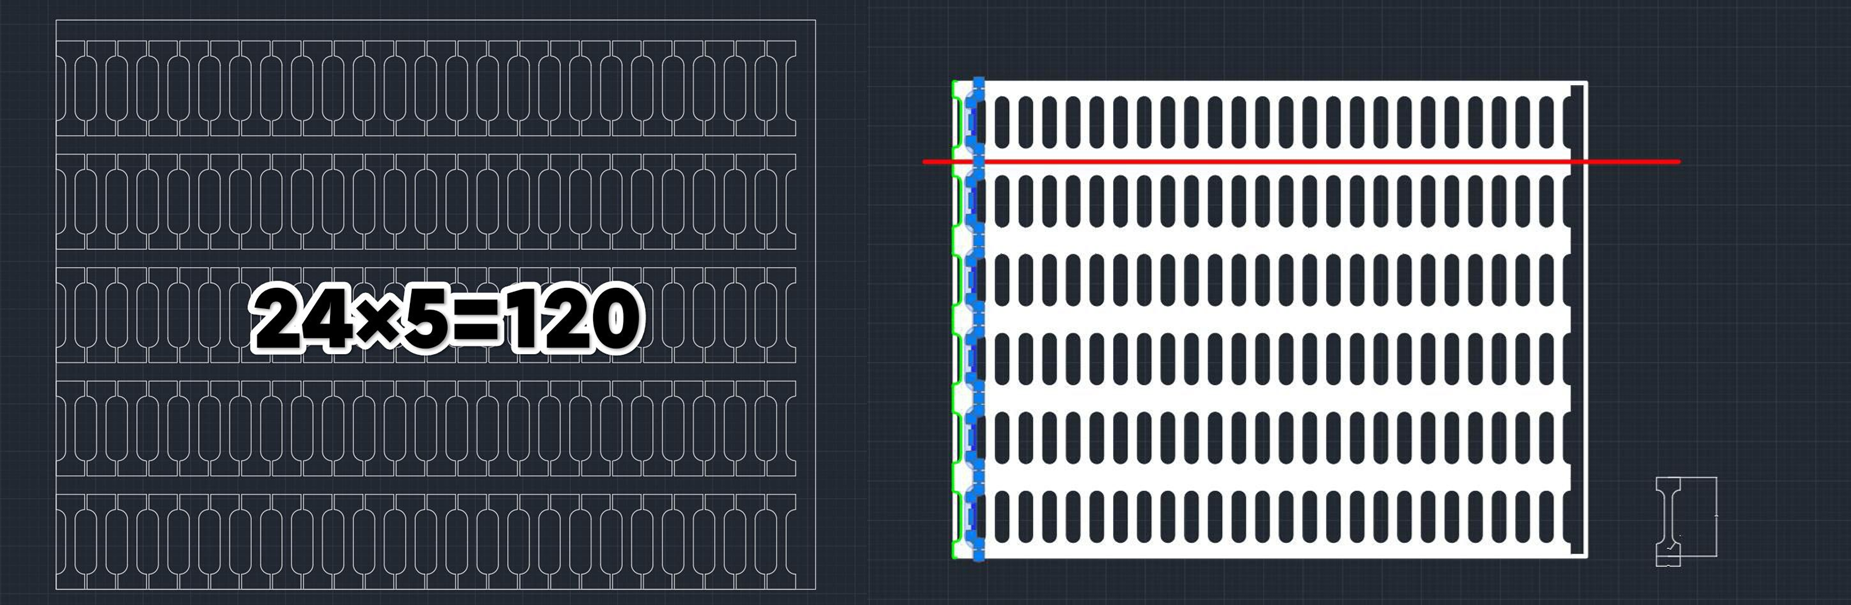
\includegraphics[width=0.8\linewidth]{pic/刀路初步}
	\caption{初步设计的刀路}
	\label{fig:badway}
\end{figure}


在仔细考虑了加工方法、设备特点、加工成本等因素后,在工程训练中心张冠老师的协助下,将加工方式改进成了:先把大板切割成八个小板,再把小板叠在一起进行加工。的方法,最终切割出来了$ 7\times 8=56 $个试样。
% TODO: \usepackage{graphicx} required
\begin{figure}[h!]
	\centering
	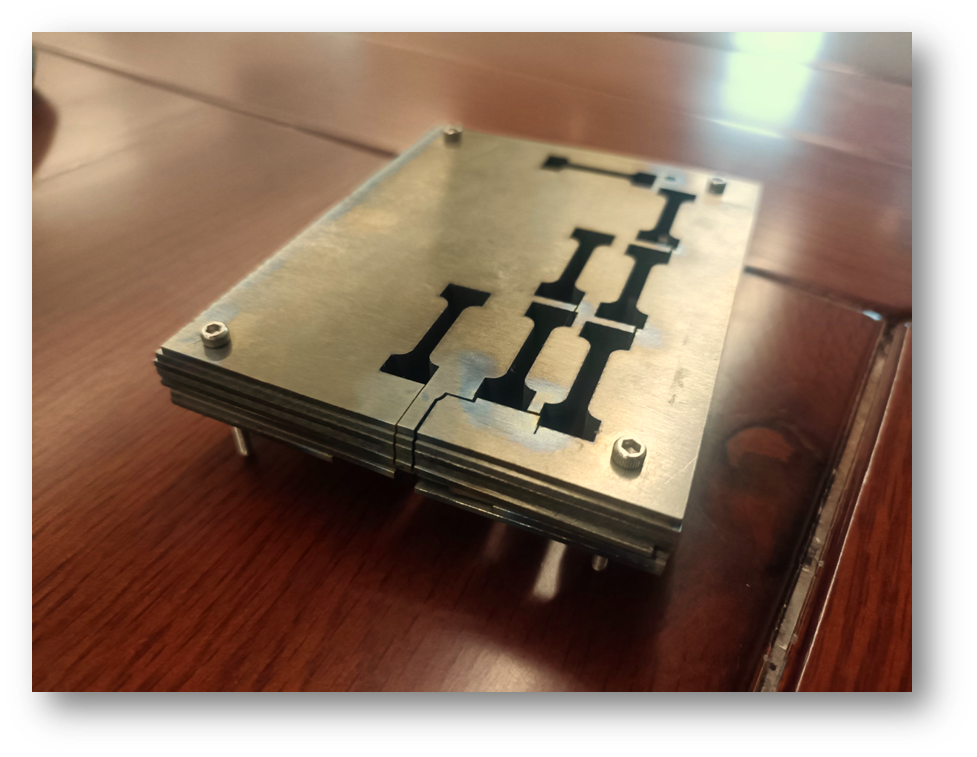
\includegraphics[width=0.7\linewidth]{pic/堆叠式切割}
	\caption{堆叠式切割}
	\label{fig:goodway}
\end{figure}


\section{TC4型钛合金的热处理工艺}
由~\ref{sec:1.1}可知,钛合金可以通过各种各样的相变过程来得到不同的组织结构。因而可以设计适宜的热处理工艺参数,来获得具有高强度的显微组织,由此实现\ti 合金力学性能和工艺性能的改善。\ti 合金热处理的一些特性如下:
\begin{enumerate}
%	\item 钛合金的热处理主要用于α+β型钛合金。因为对于纯α型钛合金而言,马氏体相变不会使钛合金的性能发生显著变化。只能依赖淬火形成的亚稳相(包括马氏体相)的时效分解来进行。
%	\item 热处理应该避免形成ω相。形成ω相会使钛合金变脆,正确选择时效工艺(例如,采用较高的时效温度)即可使相分解。
	\item α+β钛合金的淬透性差,淬火热应力大,淬火时零件易翘曲。由于导热性差,钛合金变形时易引起局部温升过高,使局部温度有可能超过β转变点而形成魏氏组织。
	\item 化学性质活泼。热处理时,钛合金易与氧和水蒸气反应,在工件表面形成具有一定深度的富氧层或氧化皮,使合金的性能降低。同时钛合金热处理时容易吸氢,引起氢脆。
	\item β转变点差异大。即使是同一成分,但由于冶炼炉次的不同,其β转变温度有时差别很大。
\end{enumerate}

常见的\ti 钛合金热处理工艺有:退火、淬火(往往加上时效处理)、形变热处理等,不同的热处理方式得到的组织性能各异。

 鲁媛媛,马保飞等人研究发现在时效温度为450、500和550℃时初生α相的含量随温度升高逐渐增加;而在时效温度为600℃和650℃条件下初生α相含量因高温溶解而明显减少, β相尺寸相应增大。当时效温度为550℃时, 所得钛合金的显微组织最佳\cite{luyuanyuanShixiaochuliduiTC4taihejinweiguanzuzhihelixuexingnengdeyingxiang2019}。刘婉颖、林元华等人通过实验发现:在960 ℃/1 h + WQ进行固溶处理和500 ℃/4 h + AC下进行时效处理得到的\ti 具有最佳的力学性能\cite{LiuWanYingBuTongReChuLiGongYiDuiTi6Al4VTaiHeJinWeiGuanJieGouHeLiXueXingNengYingXiangYingWen2017};陈冠宇通过实验表明,在850℃进行退火处理时,在600℃进行时效处理可以使合金得到更好的耐腐蚀性能\cite{1200};李宸宇证明\ti 合金在900℃空冷固溶两小时在530℃时效四小时后具有更好的强硬度,而且固溶后冷速越快,合金的强硬度越高、塑韧性越差\cite{900}。%第46页


%不同热处理作用如下:
%\begin{enumerate}
%	\item 退火:用于提高合金塑形、稳定组织。
%	\item 淬火:用于强化组织,提高综合力学性能。
%	\item 形变热处理:与压力加工结合起来,同时发挥相变强化和热处理强化的作用。
%	\item 化学热强化:提高金属耐磨性,抗腐蚀性
%\end{enumerate}

%\subsection{热处理工艺对一般钛合金组织的影响}

\section{TC4钛合金的热处理方案设计}
对于α+β型的\ti 钛合金的固溶时效热处理工艺而言,其主要影响参数为温度和时间。在研读了一些前人的研究报告\cite{mirror1}\cite{ranxingGurongwenduduiTi6Al4VELItaihejinxianweizuzhijixingnengdeyingxiang2021}之后,初步确定了固溶处理的最佳工艺制度为$ \beta $相变点以下30℃左右(这里取整数$ 947.325\simeq950^{\circ} \mathrm{C} $)处理一个小时、时效温度在450℃左右处理一个小时。于是本设计首先确定了如下三个变量:固溶温度、固溶方式、时效温度。
\subsection{正交实验设计}
用正交实验代替传统的控制变量法来提高实验效率、材料利用率。传统的控制变量法在面对低因素、低水平的实验时可以设计出很清晰直观的实验,但是面对多因素(变量)、多水平的实验时,控制变量法就显得极为繁琐了。比如一个含有三个变量,每个变量有三个水平的实验就需要$ 3\times 3 \times 3=27$次实验,为了直观性而牺牲大量的成本、同时包含了太多无关的对照组,这样的实验设计在很大程度上是不符合可持续发展理念的,是在浪费资源。但好在有另外一种方法可以解决问题——正交试验设计法(Orthogonal experimental design)。

正交实验设计是研究多因素多水平的又一种设计方法,它是根据正交性从全面试验中挑选出部分有代表性的点进行试验,这些有代表性的点具备了“均匀分散,齐整可比”的特点\cite{wangxueshen}。当实验次数太多时,根据正交实验设计,实验者可以选择一部分有代表性水平组合进行试验。 例如前面说的三因素三水平的实验,若按$ L9(3^4) $正交表安排实验,只需作9次,按$ L15(3^7) $正交表进行15次实验,显然大大减少了工作量。

在没有通过正交实验设计之前,笔者的实验是如\ref{sec:first}这样设置的:
\begin{table}[htbp]
	\centering
	\caption{\ti 原本的热处理制度设计}
	\label{sec:first}
	\begin{tabular}{cccccc}
		\toprule
		固溶温度/℃ &处理时间/h & 冷却方法 & 时效温度/℃  &处理时间/h & 冷却方法 \\
		\midrule
			910 & 1 & $\mathrm{WQ}$ & 510 & 4 & $\mathrm{AC}$\\
			910 & 1 & $\mathrm{FC}$  & 510 & 4 & $\mathrm{AC}$ \\
			910 & 1 & $\mathrm{WQ}$ & 550 & 4 & $\mathrm{AC}$ \\
			910 & 1 & $\mathrm{FC}$  & 550 & 4 & $\mathrm{AC}$ \\
			910 & 1 & $\mathrm{WQ}$ & 590 & 4 & $\mathrm{AC}$ \\
			910 & 1 & $\mathrm{FC}$  & 590 & 4 & $\mathrm{AC}$ \\
			\midrule
			950 & 1 & $\mathrm{WQ}$ & 510 & 4 & $\mathrm{AC}$ \\
			950 & 1 & $\mathrm{FC}$ & 510 & 4 & $\mathrm{AC}$ \\
			950 & 1 & $\mathrm{WQ}$ & 550 & 4 & $\mathrm{AC}$ \\
			950 & 1 & $\mathrm{FC}$ & 550 & 4 & $\mathrm{AC}$ \\
			950 & 1 & $\mathrm{WQ}$ & 590 & 4 & $\mathrm{AC}$ \\
			950 & 1 & $\mathrm{FC}$ & 590 & 4 & $\mathrm{AC}$ \\
			\midrule
			990 & 1 & $\mathrm{WQ}$ & 510 & 4 & $\mathrm{AC}$ \\
			990 & 1 & $\mathrm{FC}$ & 510 & 4 & $\mathrm{AC}$ \\
			990 & 1 & $\mathrm{WQ}$ & 550 & 4 & $\mathrm{AC}$ \\
			990 & 1 & $\mathrm{FC}$ & 550 & 4 & $\mathrm{AC}$ \\
			990 & 1 & $\mathrm{WQ}$ & 590 & 4 & $\mathrm{AC}$ \\
			990 & 1 & $\mathrm{FC}$ & 590 & 4 & $\mathrm{AC}$ \\
		\bottomrule
	\end{tabular}
\end{table}

从\ref{sec:first}可见,如果按照控制变量法设计实验,则至少需要$3\times2\times3  =18$次实验,才能穷举完所有变量各个水平之间的关系。为了给子孙后代留下天蓝、地绿、水清的美丽家园,本实验高举可持续发展理念伟大旗帜,并结合正交实验方法$\color{teal} L9.3.4 $对实验进行了优化。最终的热处理制度如下表所示\footnote{其中WQ表示水冷、FC表示炉冷、AC表示空冷。}
\begin{table}[htbp]
	\centering
	\caption{\ti 改进后的热处理制度}
	\label{sec:myHT}
	\resizebox{\linewidth}{!}{
\begin{tabular}{ccccccc}
	\toprule
		实验编号&固溶温度/℃ &处理时间/h & 冷却方法 & 时效温度/℃  &处理时间/h & 冷却方法 \\
	\midrule
	1 & 910 & 1 & 水冷 & 510 & 1 & AC \\
	2 & 910 & 1 & 油冷 & 590 & 1 & AC \\
	3 & 910 & 1 & 水冷 & 550 & 1 & AC \\
	4 & 950 & 1 & 水冷 & 590 & 1& AC \\
	5 & 950 & 1 & 水冷 & 550 & 1& AC \\
	6 & 950 & 1 & 油冷 & 510 & 1 & AC \\
	7 & 990 & 1 & 水冷 & 550 & 1 & AC \\
	8 & 990 & 1 & 油冷 & 510 & 1 & AC \\
	9 & 990 & 1 & 水冷 & 590 & 1 & AC \\
%	910 & 1 & $\mathrm{WQ}$ & 510 & 4 & $\mathrm{AC}$\\
%	910 & 1 & $\mathrm{FC}$  & 510 & 4 & $\mathrm{AC}$ \\
%	910 & 1 & $\mathrm{WQ}$ & 550 & 4 & $\mathrm{AC}$ \\
%	910 & 1 & $\mathrm{FC}$  & 550 & 4 & $\mathrm{AC}$ \\
%	910 & 1 & $\mathrm{WQ}$ & 590 & 4 & $\mathrm{AC}$ \\
%	910 & 1 & $\mathrm{FC}$  & 590 & 4 & $\mathrm{AC}$ \\
%	\midrule
%	950 & 1 & $\mathrm{WQ}$ & 510 & 4 & $\mathrm{AC}$ \\
%	950 & 1 & $\mathrm{FC}$ & 510 & 4 & $\mathrm{AC}$ \\
%	950 & 1 & $\mathrm{WQ}$ & 550 & 4 & $\mathrm{AC}$ \\
%	950 & 1 & $\mathrm{FC}$ & 550 & 4 & $\mathrm{AC}$ \\
%	950 & 1 & $\mathrm{WQ}$ & 590 & 4 & $\mathrm{AC}$ \\
%	950 & 1 & $\mathrm{FC}$ & 590 & 4 & $\mathrm{AC}$ \\
%	\midrule
%	990 & 1 & $\mathrm{WQ}$ & 510 & 4 & $\mathrm{AC}$ \\
%	990 & 1 & $\mathrm{FC}$ & 510 & 4 & $\mathrm{AC}$ \\
%	990 & 1 & $\mathrm{WQ}$ & 550 & 4 & $\mathrm{AC}$ \\
%	990 & 1 & $\mathrm{FC}$ & 550 & 4 & $\mathrm{AC}$ \\
%	990 & 1 & $\mathrm{WQ}$ & 590 & 4 & $\mathrm{AC}$ \\
%	990 & 1 & $\mathrm{FC}$ & 590 & 4 & $\mathrm{AC}$ \\
	\bottomrule
\end{tabular}
}
\end{table}

\subsection{正交实验分析方法}
经过正交实验方法设计的实验虽然节省了试验次数,但是不能兼顾直观性,因而需要专门的分析工具才能分析出来,不同变量之间的相关性,故本实验采用spssau提供的数据分析工具来对三因素影响结果进行分析。

%{\Huge \color{red} \textbf {待补充}}

\section{TC4钛合金的热处理方案实验过程}
按照\ref{sec:myHT}设置好的工艺,本实验分先后两次进行热处理:先进行固溶处理,随后进行时效处理。
\subsection{实验设备}
本次设计热处理实验所用的设备为\text{\color{teal}JC-MF12-30}型箱式电阻炉,外观如\ref{fig: mymuffle}所示,设备规格如\ref{sec:mymuffle}所示:


\begin{table}[htbp]
	\centering
	\caption{\text{\color{teal}JC-MF12-30}型箱式电阻炉的规格}
	\label{sec:mymuffle}
		\begin{tabular}{cc}
			\toprule
			参数&值\\
			\midrule
			型号&JC-MF12-30\\
			编号&803229\\
			电压&380V\\
			功率&12KW\\
			常用温度&1150℃\\
			最高温度&1200℃\\
			炉膛尺寸& 500$ \times $ 300$ \times $ 200(mm) \\
			制造日期&2023年2月\\
			制造商& $\text{青岛聚创}^\text{\textregistered}  $环保集团有限公司\\
			\bottomrule
		\end{tabular}
\end{table}

\begin{figure}[h!]
	\centering
	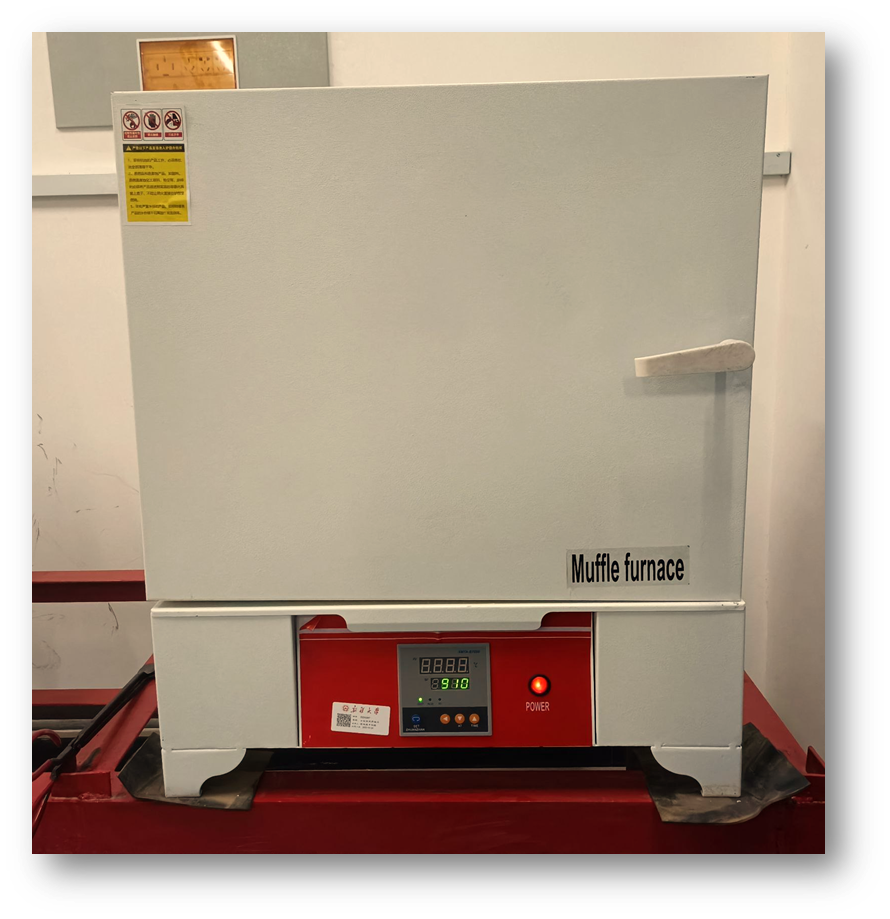
\includegraphics[width=0.7\linewidth]{pic/马弗炉}
	\caption{马弗炉外形}
	\label{fig: mymuffle}
\end{figure}

固溶实验需要淬火,用到的淬火液体如\ref{fig:淬火用液体}所示:
\begin{figure}[h!]
	\centering
	\subfigure[水淬液]{
		\label{fig:subfig:WCfluid}
		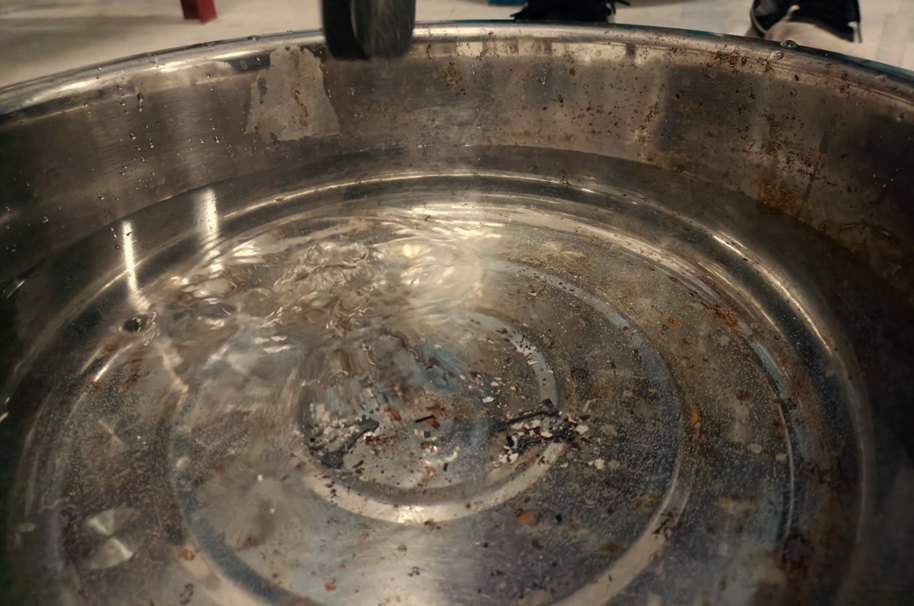
\includegraphics[scale=0.4]{pic/水淬液}}
	\hspace{0.5in} % 两图片之间的距离
	\subfigure[淬火油]{
		\label{fig:subfig:OCfluid}
		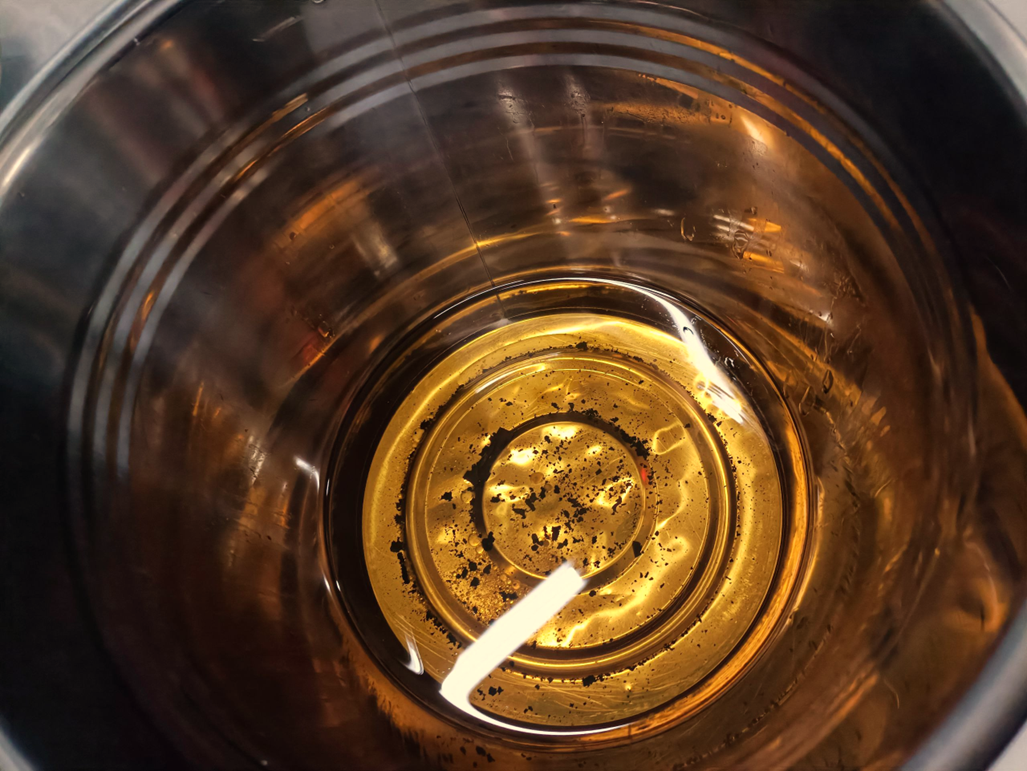
\includegraphics[scale=0.32]{pic/淬火油}}
	\caption{淬火用的液体}
	\label{fig:淬火用液体}
\end{figure}

\subsection{固溶处理实验过程}
\begin{enumerate}
	\item 设备与试样准备:把样品用去离子水等清洗干净,确保表面干净无杂质,无水分。准备陶瓷样品架,以便样品可以均匀加热。准备好后,将热处理炉预热至900℃左右,并保持稳定。
	\item 样品装入:将切好的样品用放置在样品架上,不要使样品直接接触炉子底部或顶部,以免影响加热效果。并确保样品间距均匀,并记录好摆放顺序。
	\item 加热过程控制:将样品架或钛合金网放入炉中,启动加热程序。根据实验要求,控制加热速率、温度和保温时间等参数(这里分三批次进行加热)。
	\item 保温时间控制:加热到设计的温度后后,让试样保温一段时间,使其完全进入固溶状态。保持加热系统稳定,避免温度波动。
	\item 停止加热:当固溶处理时间到达后,停止加热并关闭加热系统。
	\item 水淬或空冷:将处理后的样品快速分别浸入水中、淬火油中进行淬火。
	\item 后处理:取出样品进行干燥、清洗、归类,并记录初步记录数据。
\end{enumerate}
经过固溶时效处理后的试样如图所示:



%\section{小结}
%在本节中,介绍了式样的参数与加工过程与热处理工艺的设计

	\chapter{力学性能实验与组织表征}

\section{TC4钛合金的力学实验过程}
力学性能是表征材料性能的重要参数,本实验采用常规的拉伸试验来测量式样的力学性能。测量的包括屈服强度、抗拉强度。

本设计采用拉伸试验机对经固溶时效热处理工艺的试样进行常温微拉伸性能测试,拉伸速率为$ 2mm/min $,每组试样进行两次测定,取其平均值。

为了节约成本,本设计选择了尺寸较小的试样来进行实验,整体尺寸为$ 25mm\times 7.5mm $的狗骨状片体,具体参数如\ref{fig:试样尺寸}所示:
%3-28日上午,经过老师说明,由于试样为板材,加工成圆柱较为困难,故加工成二位平面的“狗骨头”

\begin{figure}[h!]
	\centering
	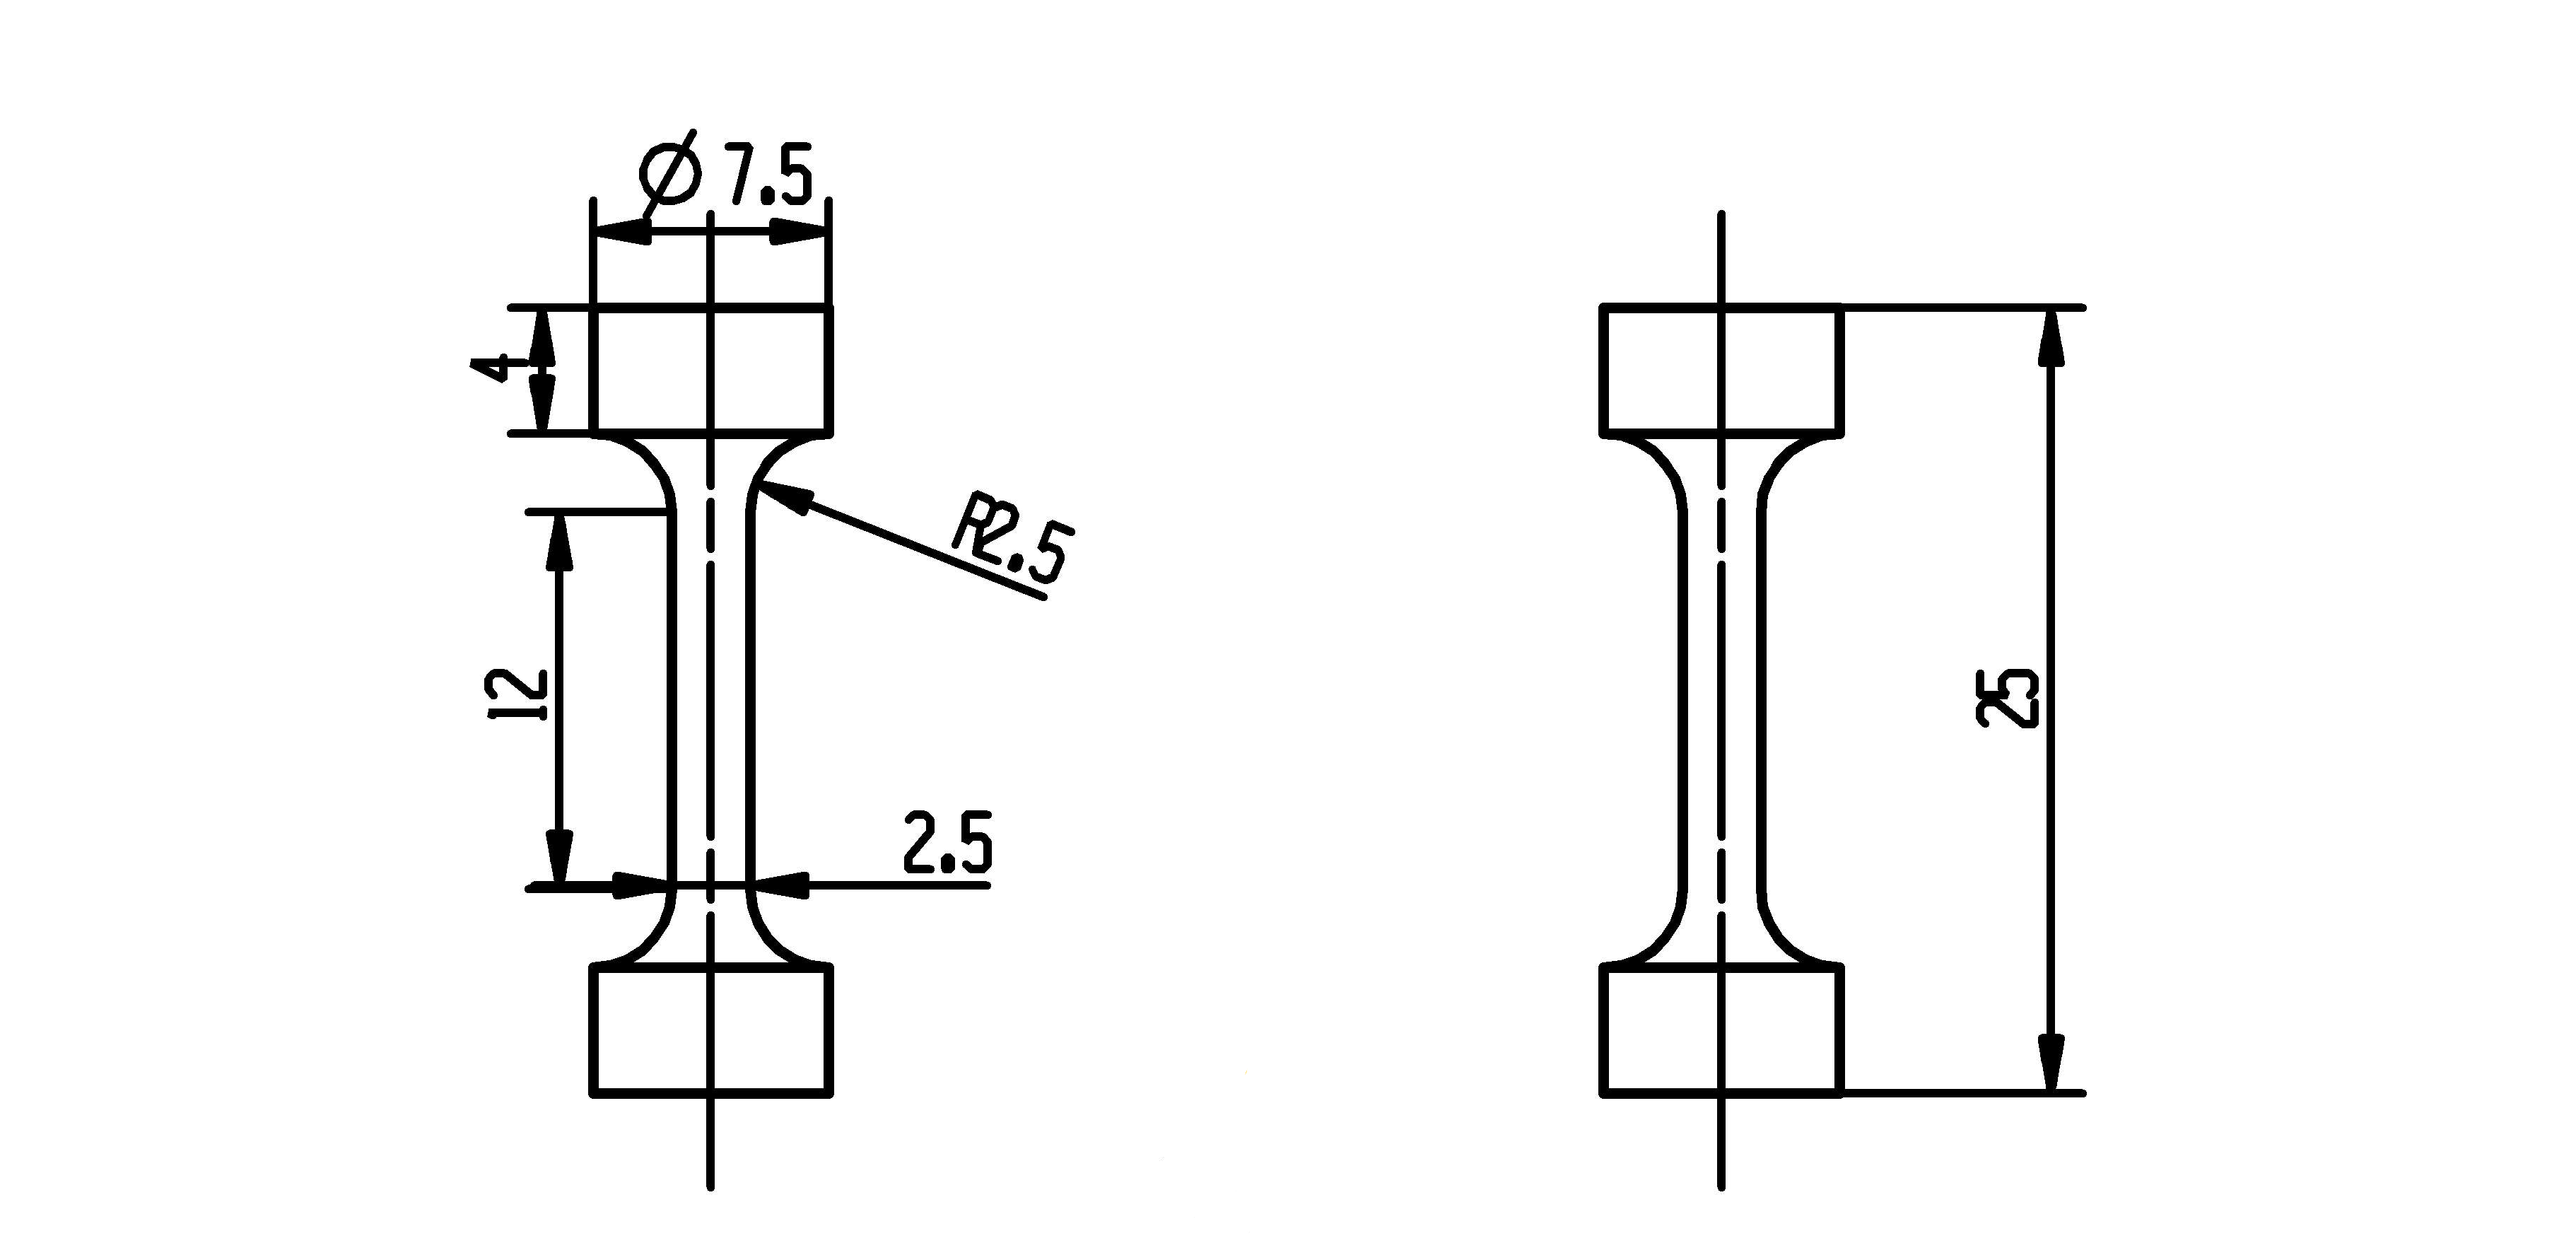
\includegraphics[width=0.99\linewidth]{pic/试样}
	\caption{试样的尺寸参数}
	\label{fig:试样尺寸}
\end{figure}


在某型号万能力学试验机上测试得到的结果如下:

\begin{table}[htbp]
	\centering
	\caption{\ti 合金的力学性能实验结果}
	\label{sec:mystrength}
		\begin{tabular}{ccc}
			\toprule
			实验编号&$ R_m $/Mpa&$ R_{p0.2} $/Mpa \\
			\midrule
			1 & 950 & 866\\
			2 & 946 & 872\\
			3 & 976 & 884\\
			4 & 988 & 894\\
			5 & 990 & 920\\
			6 & 972 & 886\\
			7 & 966 & 820\\
			8 & 978 & 849\\
			9 & 959 & 836\\
			\bottomrule
		\end{tabular}
\end{table}
\newpage
\section{TC4钛合金的显微组织表征}
试验期间用来观察组织和分析相结构的检测方法,主要包括光学显微镜 (OM)、扫描式电子显微镜 (SEM)、X射线衍射分析 (XRD)以及透射式电子显微镜 (TEM)等。

将固溶与时效后的试件进行线切割截取显微组织分析试样,截取后的试样进行 150\#、400\#、1000\#、1500\#、2000\#、2500\#金相砂纸磨制,对磨制后的试样采用 0.05umSiO2抛光液在抛光机上进行抛光,去除试样表面的划痕或杂质颗粒,经抛光后的试样采用$ HF:HNO3:H2O=2:4:94 $的Kroll试剂进行腐蚀。腐蚀后的试样分别采用光 学显微镜(OM)、扫描电子显微镜(SEM)对其微观形貌进行观察。


三种不同固溶温度得到的试样组织如下:
\begin{figure}[h!]
	\centering
	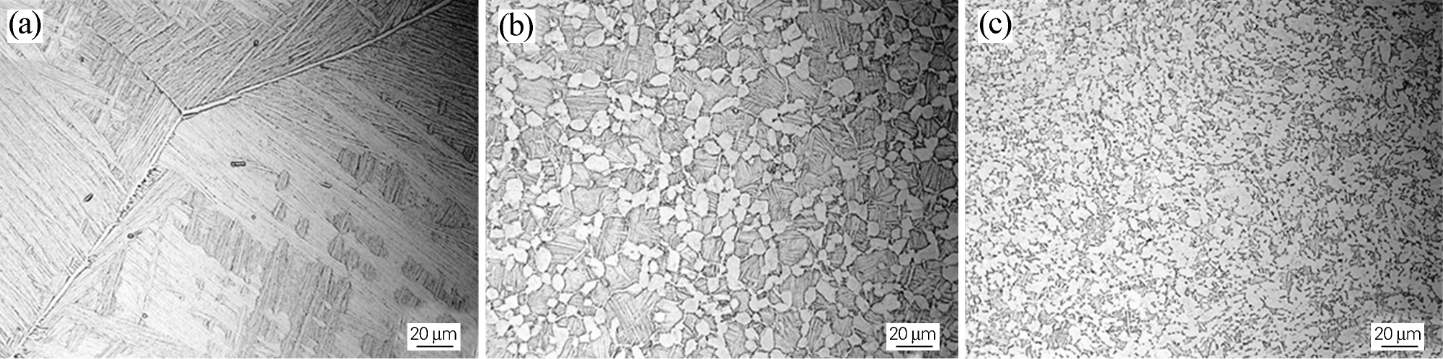
\includegraphics[width=0.7\linewidth]{pic/demo-mico}
	\caption{不同热处理工艺下 TC4 钛合金的显微组织}
	\label{fig:demo-mico}
\end{figure}
	\chapter{综合分析}
不同的组织会使材料表现出来不同的性能。
\section{基于机器学习的金相组织分析}
\section{性能与热处理的关系}
\section{微观机理}
\section{结论}


	\backmatter
	\listoffigures
	\listoftables
	\clearpage
	\phantomsection
	\addcontentsline{toc}{chapter}{参考文献}
	\bibliography{ciiiiiiiiite}

\end{document}


